\UseRawInputEncoding
\documentclass{beamer}
\usetheme{Madrid}
\usepackage{listings}
\usepackage[utf8]{inputenc}
\usepackage{graphicx}
\usepackage{booktabs}
\usepackage{xcolor} % Added for color support in listings
\usepackage{multirow}
\usepackage{tikz}
\usetikzlibrary{shapes,arrows,positioning}
\usepackage{pgfplots}
\pgfplotsset{compat=1.18}

\lstset{
  language=Python,
  basicstyle=\tiny\ttfamily,
  keywordstyle=\color{blue},
  stringstyle=\color{red},
  commentstyle=\color{green},
  breaklines=true
}


\title{Introduction to Linear Programming}
\subtitle{BUS 104: Decision Analysis and Management Science}
\author{Danko Turcic}
\titlegraphic{\includegraphics[width=5cm]{UCR-Logo.jpg}}


\begin{document}

% The \maketitle command should be inside a frame
\begin{frame}[noframenumbering,plain]
  \maketitle
\end{frame}


\begin{frame}
\frametitle{Agenda: Linear Programming Applications}
\textbf{Welcome!} In this presentation, we will explore the power of Linear Programming (LP) through a series of foundational business and operational problems. 

\vspace{0.3cm}
We will cover how to formulate and solve:
\begin{enumerate}
    \item \textbf{Product Mix Problem:} Maximizing manufacturing profit (Par, Inc.)
    \item \textbf{Blending Problems (I \& II):} Mixing ingredients to meet specifications at lowest cost (e.g., Coffee Blending)
    \item \textbf{Work Scheduling Problem:} Assigning labor shifts to meet demand
    \item \textbf{Transportation Problem:} Minimizing shipping costs from origins to destinations
    \item \textbf{Assignment Problem:} Optimal 1-to-1 resource allocation (e.g., Project Staffing)
    \item \textbf{Shortest Path Problem:} Finding the most efficient route through a network
\end{enumerate}
\end{frame}

\begin{frame}
\frametitle{Our Approach}
For each problem category, we will follow a rigorous 3-step methodology:
\vspace{0.5cm}
\begin{itemize}
    \item \textbf{Step 1: The Business Problem.} Understanding the scenario, the physical constraints, and the managerial objective.
    \item \textbf{Step 2: Mathematical Formulation.} Translating English into Algebra (defining Decision Variables, Objective Function, and Constraints).
    \item \textbf{Step 3: Python Implementation.} Using the \texttt{PuLP} library to computationally solve the model and extract business insights.
\end{itemize}
\vspace{0.5cm}
Let's begin with our first category: The Product Mix Problem.
\end{frame}


% Slide from BUS104-Lectures_3_4.pptx.pdf Page 1
\begin{frame}
\frametitle{Product Mix Example: Par, Inc.}
\textbf{Goal:} Maximize weekly profit by deciding how many standard and deluxe golf bags to produce.

\vspace{0.3cm}
\textbf{The Data:}
\begin{center}
\renewcommand{\arraystretch}{1.2}
\begin{tabular}{|l|c|c|c|}
\hline
\textbf{Department} & \textbf{Standard Bag} & \textbf{Deluxe Bag} & \textbf{Hours Available} \\
\hline
Cutting \& Dyeing & 7/10 hr & 1 hr & 630 hrs \\
Sewing & 1/2 hr & 5/6 hr & 600 hrs \\
Finishing & 1 hr & 2/3 hr & 708 hrs \\
Inspection \& Pack. & 0.1 hr & 1/4 hr & 135 hrs \\
\hline
\textbf{Profit/Bag} & \textbf{\$10} & \textbf{\$9} & \\
\hline
\end{tabular}
\end{center}

\vspace{0.3cm}
\begin{itemize}
    \item \textit{Assumption:} Demand is unlimited; we can sell everything we make.
    \item \textbf{Question:} Formulate a mathematical model to find the optimal production plan.
\end{itemize}
\end{frame}


\begin{frame}[shrink]{Par, Inc. Golf Bag Production Problem}

\textbf{Decision variables.} \\
Let \(x_s\) = number of standard golf bags produced per week,\\
and \(x_d\) = number of deluxe golf bags produced per week.\\[1ex]
Both \(x_s, x_d \ge 0.\)
\pause\\
\bigskip
\textbf{Objective function.} \\
Maximize weekly profit:
\[
\max \; Z = 10x_s + 9x_d.
\]

\textbf{Subject to capacity constraints:}
\[
\begin{aligned}
\tfrac{7}{10}x_s + 1x_d &\le 630 &\text{(Cutting \& Dyeing)}\\\pause
\tfrac{1}{2}x_s + \tfrac{5}{6}x_d &\le 600 &\text{(Sewing)}\\\pause
1x_s + \tfrac{2}{3}x_d &\le 708 &\text{(Finishing)}\\\pause
0.1x_s + \tfrac{1}{4}x_d &\le 135 &\text{(Inspection \& Packaging)}\\
x_s, x_d &\ge 0.
\end{aligned}
\]
\end{frame}

\begin{frame}[fragile, shrink]
\frametitle{Par, Inc. Golf Bag Production Solution (PuLP)}
\begin{lstlisting}
import pulp as pl

# Create the problem
prob = pl.LpProblem("Par_Inc_Golf_Bags", pl.LpMaximize)

# Define variables directly into the model
x_s = prob.add_variable("Standard_Bags", lowBound=0)
x_d = prob.add_variable("Deluxe_Bags", lowBound=0)

# Objective function
prob += 10 * x_s + 9 * x_d, "Maximize_Profit"

# Constraints
prob += 0.7 * x_s + 1 * x_d <= 630, "Cutting_Dyeing"
prob += 0.5 * x_s + 5/6 * x_d <= 600, "Sewing"
prob += 1 * x_s + 2/3 * x_d <= 708, "Finishing"
prob += 0.1 * x_s + 0.25 * x_d <= 135, "Inspection_Packaging"

# Solve the problem
res = prob.solve()

# Print results
print("Status:", res.status.name)
print("Optimal Solution:")
print(f"Standard Bags = {x_s.varValue}")
print(f"Deluxe Bags = {x_d.varValue}")
print(f"Maximum Profit = ${pl.value(prob.objective)}")
\end{lstlisting}
\end{frame}



\begin{frame}
\frametitle{Graphical Solution -- Step 1: Set up the Axes}
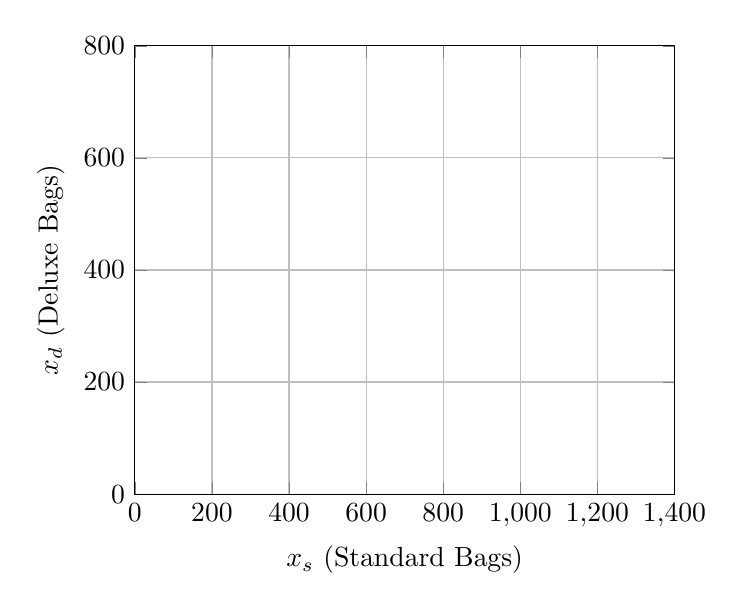
\begin{tikzpicture}
\begin{axis}[
  xlabel={\(x_s\) (Standard Bags)},
  ylabel={\(x_d\) (Deluxe Bags)},
  xmin=0, xmax=1400,
  ymin=0, ymax=800,
  grid=major,
]
\end{axis}
\end{tikzpicture}
\end{frame}


\begin{frame}
\frametitle{Graphical Solution -- Step 2: Add C\&D Constraint}
\vspace{-0.25cm}
\(0.7 x_s + x_d \leq 630\)
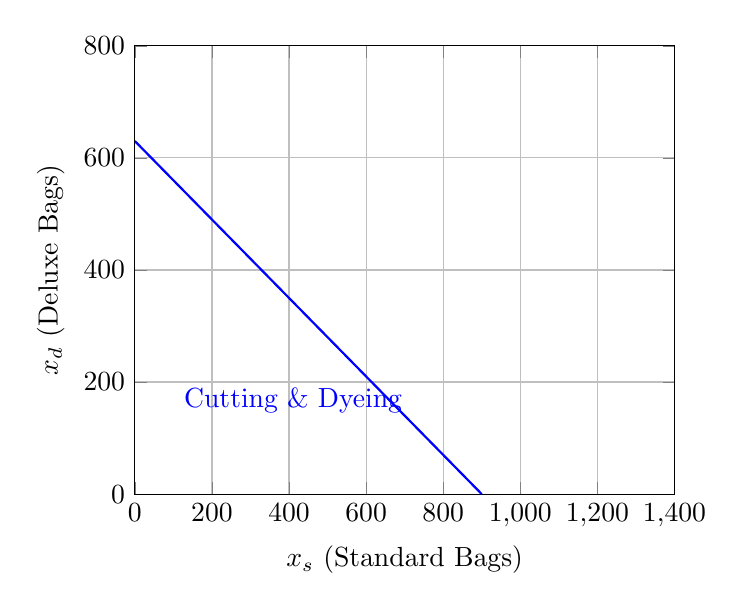
\begin{tikzpicture}
\begin{axis}[
  xlabel={\(x_s\) (Standard Bags)},
  ylabel={\(x_d\) (Deluxe Bags)},
  xmin=0, xmax=1400,
  ymin=0, ymax=800,
  grid=major,
]
\addplot[thick, blue, domain=0:900] {630 - 0.7*x} node[pos=0.8, above left] {Cutting \& Dyeing};
\end{axis}
\end{tikzpicture}
Feasible region is below the line.
\end{frame}

\begin{frame}
\frametitle{Graphical Solution -- Step 3: Add Sewing Constraint}
\(0.5 x_s + \frac{5}{6} x_d \leq 600\)
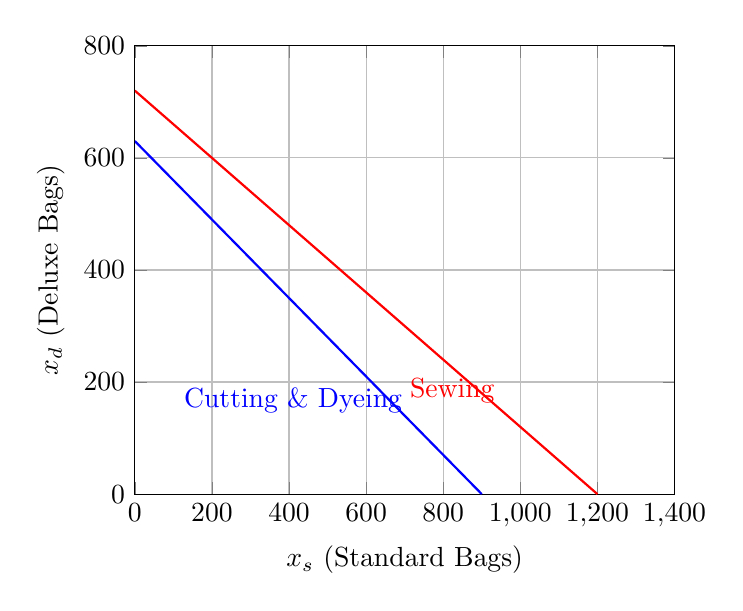
\begin{tikzpicture}
\begin{axis}[
  xlabel={\(x_s\) (Standard Bags)},
  ylabel={\(x_d\) (Deluxe Bags)},
  xmin=0, xmax=1400,
  ymin=0, ymax=800,
  grid=major,
]
\addplot[thick, blue, domain=0:900] {630 - 0.7*x} node[pos=0.8, above left] {Cutting \& Dyeing};
\addplot[thick, red, domain=0:1200] {720 - 0.6*x} node[pos=0.8, above left] {Sewing};
\end{axis}
\end{tikzpicture}
Feasible region is below the line.
\end{frame}

\begin{frame}
\frametitle{Graphical Solution -- Step 4: Add Finishing Constraint}
\(x_s + \frac{2}{3} x_d \leq 708\)
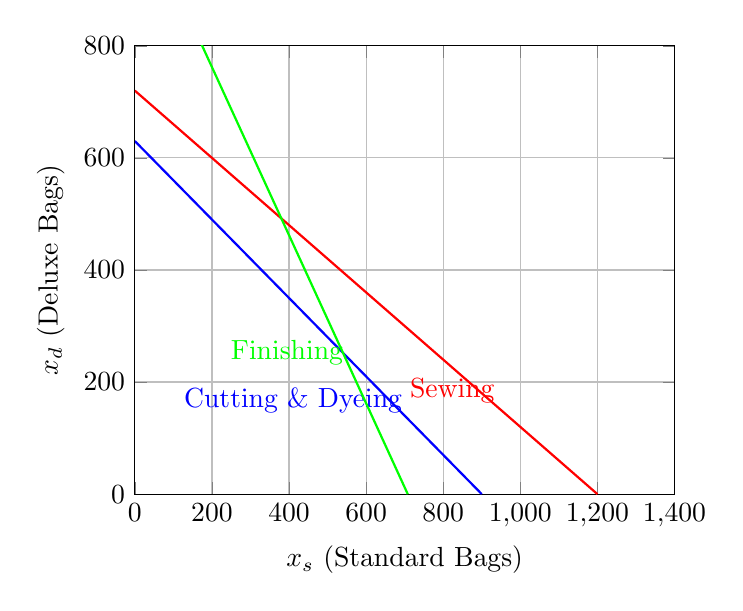
\begin{tikzpicture}
\begin{axis}[
  xlabel={\(x_s\) (Standard Bags)},
  ylabel={\(x_d\) (Deluxe Bags)},
  xmin=0, xmax=1400,
  ymin=0, ymax=800,
  grid=major,
]
\addplot[thick, blue, domain=0:900] {630 - 0.7*x} node[pos=0.8, above left] {Cutting \& Dyeing};
\addplot[thick, red, domain=0:1200] {720 - 0.6*x} node[pos=0.8, above left] {Sewing};
\addplot[thick, green, domain=0:708] {1062 - 1.5*x} node[pos=0.8, above left] {Finishing};
\end{axis}
\end{tikzpicture}
Feasible region is below the line.
\end{frame}

\begin{frame}
\frametitle{Graphical Solution -- Step 5: Add Inspection Constraint}
\(0.1 x_s + 0.25 x_d \leq 135\)
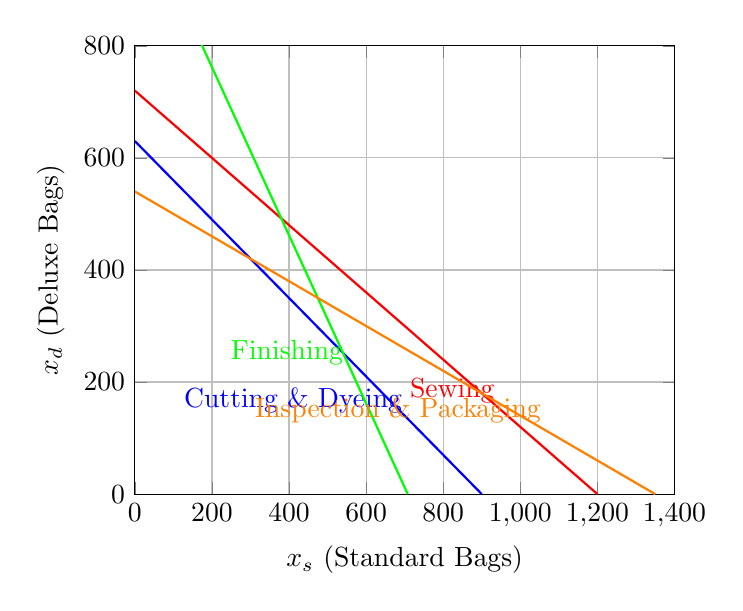
\begin{tikzpicture}
\begin{axis}[
  xlabel={\(x_s\) (Standard Bags)},
  ylabel={\(x_d\) (Deluxe Bags)},
  xmin=0, xmax=1400,
  ymin=0, ymax=800,
  grid=major,
]
\addplot[thick, blue, domain=0:900] {630 - 0.7*x} node[pos=0.8, above left] {Cutting \& Dyeing};
\addplot[thick, red, domain=0:1200] {720 - 0.6*x} node[pos=0.8, above left] {Sewing};
\addplot[thick, green, domain=0:708] {1062 - 1.5*x} node[pos=0.8, above left] {Finishing};
\addplot[thick, orange, domain=0:1350] {540 - 0.4*x} node[pos=0.8, above left] {Inspection \& Packaging};
\end{axis}
\end{tikzpicture}
Feasible region is below the line.
\end{frame}

\begin{frame}
\frametitle{Graphical Solution -- Step 6: Feasible Region}
The feasible region is the area below all constraint lines and above the axes.
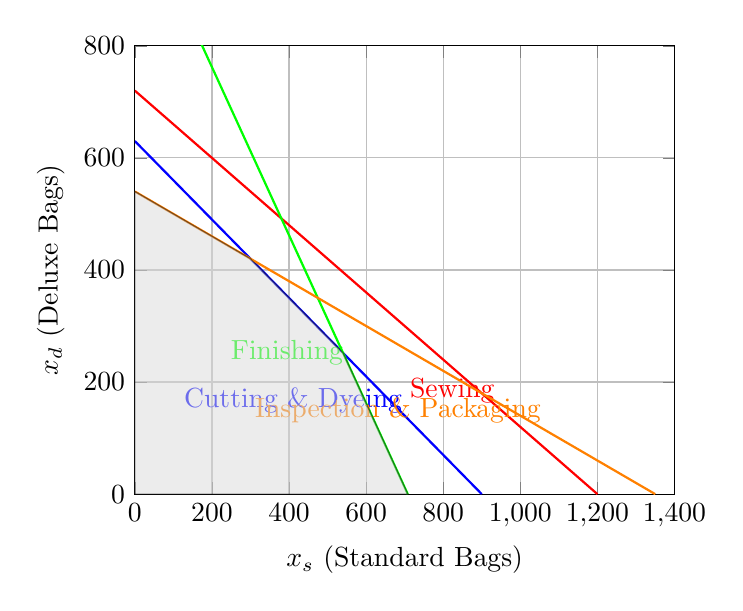
\begin{tikzpicture}
\begin{axis}[
  xlabel={\(x_s\) (Standard Bags)},
  ylabel={\(x_d\) (Deluxe Bags)},
  xmin=0, xmax=1400,
  ymin=0, ymax=800,
  grid=major,
]
\addplot[thick, blue, domain=0:900] {630 - 0.7*x} node[pos=0.8, above left] {Cutting \& Dyeing};
\addplot[thick, red, domain=0:1200] {720 - 0.6*x} node[pos=0.8, above left] {Sewing};
\addplot[thick, green, domain=0:708] {1062 - 1.5*x} node[pos=0.8, above left] {Finishing};
\addplot[thick, orange, domain=0:1350] {540 - 0.4*x} node[pos=0.8, above left] {Inspection \& Packaging};

\addplot[fill=gray!30, opacity=0.5] coordinates {
  (0,0)
  (708,0)
  (540,252)
  (300,420)
  (0,540)
} -- cycle;
\end{axis}
\end{tikzpicture}
\end{frame}


\begin{frame}
\frametitle{Graphical Solution -- Step 7: Corner Points}
Identify the corner points of the feasible region:
- (0, 0)
- (0, 540)
- (300, 420)
- (540, 252)
- (708, 0)
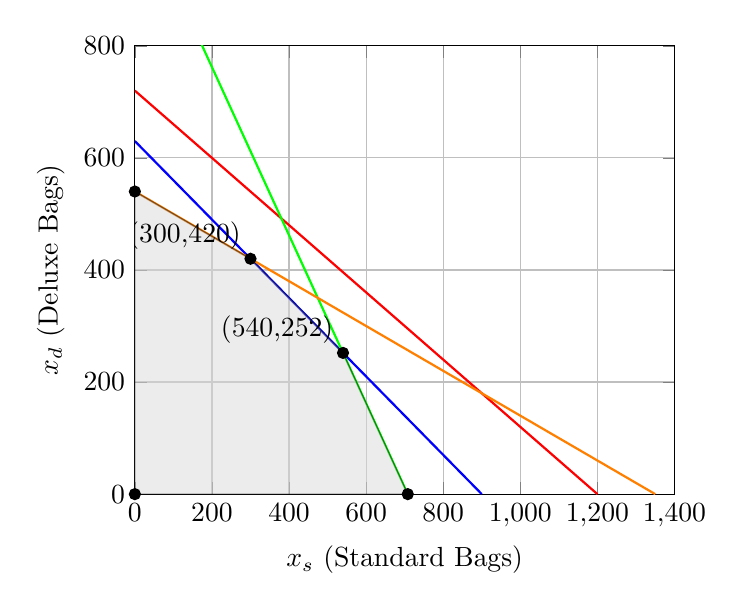
\begin{tikzpicture}
\begin{axis}[
  xlabel={\(x_s\) (Standard Bags)},
  ylabel={\(x_d\) (Deluxe Bags)},
  xmin=0, xmax=1400,
  ymin=0, ymax=800,
  grid=major,
]
\addplot[thick, blue, domain=0:900] {630 - 0.7*x};
\addplot[thick, red, domain=0:1200] {720 - 0.6*x};
\addplot[thick, green, domain=0:708] {1062 - 1.5*x};
\addplot[thick, orange, domain=0:1350] {540 - 0.4*x};

\addplot[fill=gray!30, opacity=0.5] coordinates {
  (0,0)
  (708,0)
  (540,252)
  (300,420)
  (0,540)
} -- cycle;

\addplot[mark=*, only marks] coordinates {(0,0) (0,540) (300,420) (540,252) (708,0)};
\node at (axis cs:0,0) [anchor=north west] {(0,0)};
\node at (axis cs:0,540) [anchor=south east] {(0,540)};
\node at (axis cs:300,420) [anchor=south east] {(300,420)};
\node at (axis cs:540,252) [anchor=south east] {(540,252)};
\node at (axis cs:708,0) [anchor=north west] {(708,0)};
\end{axis}
\end{tikzpicture}
\end{frame}

\begin{frame}
\frametitle{Graphical Solution -- Step 8: Objective Function at Low Profit}
Objective: \(Z = 10 x_s + 9 x_d = 4000\)
Line: \(x_d = \frac{4000}{9} - \frac{10}{9} x_s \approx 444.44 - 1.111 x_s\)
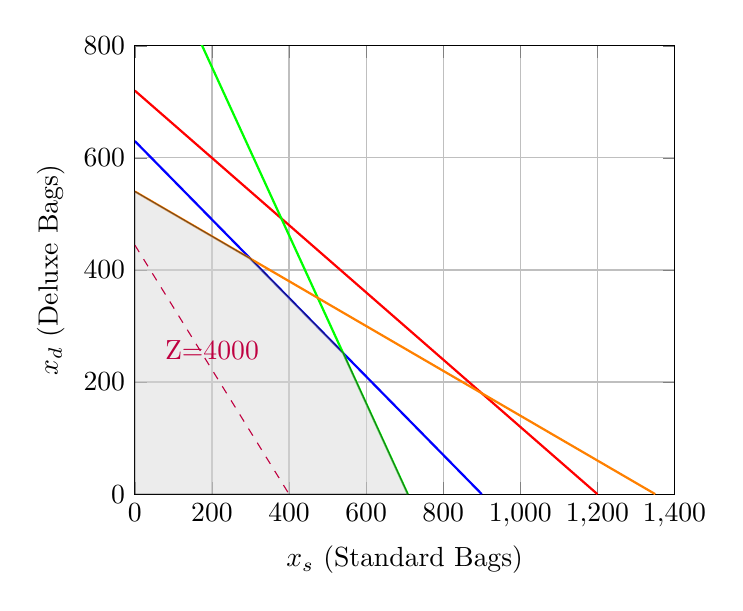
\begin{tikzpicture}
\begin{axis}[
  xlabel={\(x_s\) (Standard Bags)},
  ylabel={\(x_d\) (Deluxe Bags)},
  xmin=0, xmax=1400,
  ymin=0, ymax=800,
  grid=major,
]
\addplot[thick, blue, domain=0:900] {630 - 0.7*x};
\addplot[thick, red, domain=0:1200] {720 - 0.6*x};
\addplot[thick, green, domain=0:708] {1062 - 1.5*x};
\addplot[thick, orange, domain=0:1350] {540 - 0.4*x};

\addplot[fill=gray!30, opacity=0.5] coordinates {
  (0,0)
  (708,0)
  (540,252)
  (300,420)
  (0,540)
} -- cycle;

\addplot[dashed, purple, domain=0:4000/10] {444.44 - 1.111*x} node[pos=0.5, above] {Z=4000};
\end{axis}
\end{tikzpicture}
\end{frame}

\begin{frame}
\frametitle{Graphical Solution -- Step 9: Objective Function at Higher Profit}
Objective: \(Z = 10 x_s + 9 x_d = 6000\)
Line: \(x_d = \frac{6000}{9} - \frac{10}{9} x_s \approx 666.67 - 1.111 x_s\)
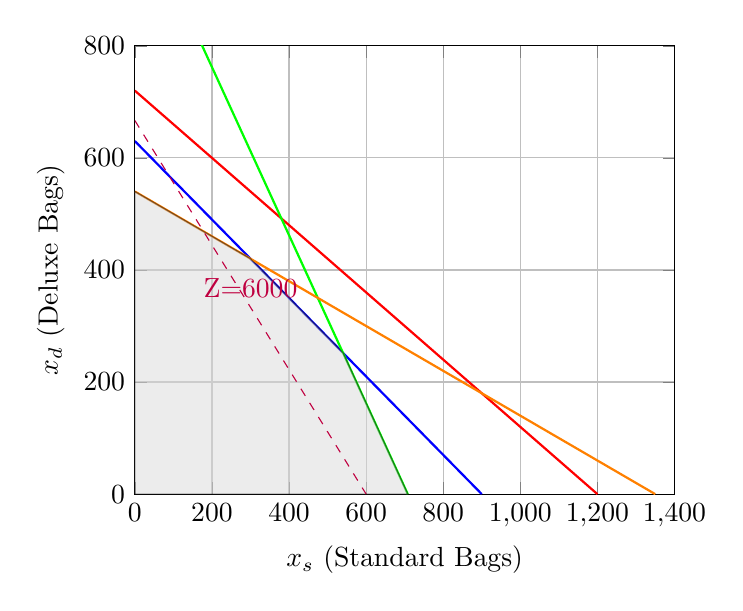
\begin{tikzpicture}
\begin{axis}[
  xlabel={\(x_s\) (Standard Bags)},
  ylabel={\(x_d\) (Deluxe Bags)},
  xmin=0, xmax=1400,
  ymin=0, ymax=800,
  grid=major,
]
\addplot[thick, blue, domain=0:900] {630 - 0.7*x};
\addplot[thick, red, domain=0:1200] {720 - 0.6*x};
\addplot[thick, green, domain=0:708] {1062 - 1.5*x};
\addplot[thick, orange, domain=0:1350] {540 - 0.4*x};

\addplot[fill=gray!30, opacity=0.5] coordinates {
  (0,0)
  (708,0)
  (540,252)
  (300,420)
  (0,540)
} -- cycle;

\addplot[dashed, purple, domain=0:6000/10] {666.67 - 1.111*x} node[pos=0.5, above] {Z=6000};
\end{axis}
\end{tikzpicture}
\end{frame}

\begin{frame}
\frametitle{Graphical Solution -- Step 10: Optimal Objective Function}
Objective: \(Z = 10 x_s + 9 x_d = 7668\)
Line: \(x_d = \frac{7668}{9} - \frac{10}{9} x_s \approx 852 - 1.111 x_s\)
The line touches the feasible region at the optimal point (540, 252).
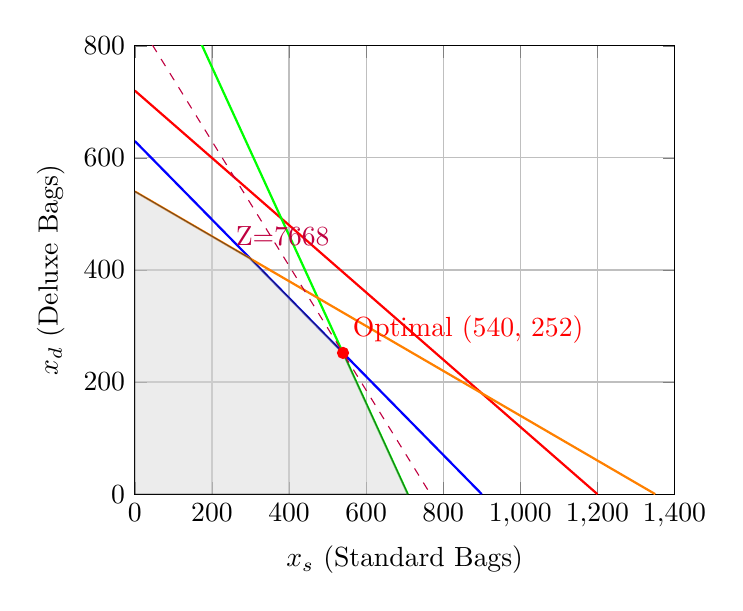
\begin{tikzpicture}
\begin{axis}[
  xlabel={\(x_s\) (Standard Bags)},
  ylabel={\(x_d\) (Deluxe Bags)},
  xmin=0, xmax=1400,
  ymin=0, ymax=800,
  grid=major,
]
\addplot[thick, blue, domain=0:900] {630 - 0.7*x};
\addplot[thick, red, domain=0:1200] {720 - 0.6*x};
\addplot[thick, green, domain=0:708] {1062 - 1.5*x};
\addplot[thick, orange, domain=0:1350] {540 - 0.4*x};

\addplot[fill=gray!30, opacity=0.5] coordinates {
  (0,0)
  (708,0)
  (540,252)
  (300,420)
  (0,540)
} -- cycle;

\addplot[dashed, purple, domain=0:7668/10] {852 - 1.111*x} node[pos=0.5, above] {Z=7668};

\addplot[mark=*, red] coordinates {(540,252)} node[above right] {Optimal (540, 252)};
\end{axis}
\end{tikzpicture}
\end{frame}






% Slide from BUS104-Lectures_3_4.pptx.pdf Page 2
\begin{frame}
\frametitle{Blending Example: MediBlend}
\textbf{Goal:} Find the cheapest way to produce today's batch of MediBlend by mixing four chemicals.

\vspace{0.2cm}
\textbf{The Rules \& Constraints:}
\begin{itemize}
    \item \textbf{Batch Size:} Must produce \textit{at least} 1,000 lbs total.
    \item \textbf{Ingredient Minimums:} The final mix must contain at least 8\% of A, 4\% of B, and 2\% of C (by weight).
    \item \textbf{Supply Constraint:} Must use \textit{at least} 100 lbs of Chemical 2.
\end{itemize}

\vspace{0.2cm}
\textbf{The Data:}
\begin{center}
\renewcommand{\arraystretch}{1.2}
\begin{tabular}{|l|c|c|c|c|}
\hline
\textbf{Chemical} & \textbf{Cost/lb} & \textbf{Ingredient A} & \textbf{Ingredient B} & \textbf{Ingredient C} \\
\hline
Chemical 1 & \$8 & 0.03 & 0.02 & 0.01 \\
Chemical 2 & \$10 & 0.06 & 0.04 & 0.01 \\
Chemical 3 & \$11 & 0.10 & 0.03 & 0.04 \\
Chemical 4 & \$14 & 0.12 & 0.09 & 0.04 \\
\hline
\end{tabular}
\end{center}
\end{frame}

\begin{frame}[shrink]
\frametitle{Blending Example: LP Formulation}
Let \(x_1,x_2,x_3,x_4\) denote the pounds of chemicals (1,2,3,4) used to produce today’s batch. The objective is to minimize total cost subject to meeting the minimum batch size, the ingredient percentage requirements, the minimum usage of chemical 2, and nonnegativity:
\pause
\[
\begin{aligned}
\min_{x_1,x_2,x_3,x_4}\quad
& 8x_1 + 10x_2 + 11x_3 + 14x_4 \\[0.5ex]\pause
\text{s.t.}\quad
& x_1 + x_2 + x_3 + x_4 \ge 1000\\\pause
& 0.03x_1 + 0.06x_2 + 0.10x_3 + 0.12x_4 \ge 0.08(x_1+x_2+x_3+x_4)\\\pause
& 0.02x_1 + 0.04x_2 + 0.03x_3 + 0.09x_4 \ge 0.04(x_1+x_2+x_3+x_4)\\\pause
& 0.01x_1 + 0.01x_2 + 0.04x_3 + 0.04x_4 \ge 0.02(x_1+x_2+x_3+x_4)\\\pause
& x_2 \ge 100 \\\pause
& x_1, x_2, x_3, x_4 \ge 0
\end{aligned}
\]
\end{frame}

\begin{frame}[shrink]
\frametitle{Blending Example: Classical LP Formulation}
In classical Linear Programming (and for many solvers), we rearrange our equations so that all variables are on the left side of the inequality, and all constants are on the right side.

\vspace{0.3cm}
By factoring out the variables from the right side of our ingredient constraints, our model simplifies to:
\[
\begin{aligned}
\min_{x_1,x_2,x_3,x_4}\quad
& 8x_1 + 10x_2 + 11x_3 + 14x_4 \\[0.5ex]
\text{s.t.}\quad
& x_1 + x_2 + x_3 + x_4 \ge 1000 & \text{(Batch Size)}\\
& -0.05x_1 - 0.02x_2 + 0.02x_3 + 0.04x_4 \ge 0 & \text{(Ingredient A)}\\
& -0.02x_1 - 0.01x_3 + 0.05x_4 \ge 0 & \text{(Ingredient B)}\\
& -0.01x_1 - 0.01x_2 + 0.02x_3 + 0.02x_4 \ge 0 & \text{(Ingredient C)}\\
& x_2 \ge 100 & \text{(Chemical 2 Min)}\\
& x_1, x_2, x_3, x_4 \ge 0
\end{aligned}
\]
\end{frame}

\begin{frame}[fragile, shrink]
\frametitle{Blending Example Solution (PuLP)}
\begin{lstlisting}
import pulp as pl

# Create the problem
prob = pl.LpProblem("MediBlend_Blending", pl.LpMinimize)

# Define variables directly into the model
x1 = prob.add_variable("Chemical_1", lowBound=0)
x2 = prob.add_variable("Chemical_2", lowBound=0)
x3 = prob.add_variable("Chemical_3", lowBound=0)
x4 = prob.add_variable("Chemical_4", lowBound=0)

# Objective function
prob += 8 * x1 + 10 * x2 + 11 * x3 + 14 * x4, "Minimize_Cost"

# Constraints
prob += x1 + x2 + x3 + x4 >= 1000, "Batch_Size"
prob += 0.03 * x1 + 0.06 * x2 + 0.10 * x3 + 0.12 * x4 >= 0.08 * (x1 + x2 + x3 + x4), "Ingredient_A"
prob += 0.02 * x1 + 0.04 * x2 + 0.03 * x3 + 0.09 * x4 >= 0.04 * (x1 + x2 + x3 + x4), "Ingredient_B"
prob += 0.01 * x1 + 0.01 * x2 + 0.04 * x3 + 0.04 * x4 >= 0.02 * (x1 + x2 + x3 + x4), "Ingredient_C"
prob += x2 >= 100, "Chemical_2_Min"

# Solve the problem
res = prob.solve()

# Print results
print("Status:", res.status.name)
print("Optimal Solution:")
print(f"Chemical 1 = {x1.varValue} lbs")
print(f"Chemical 2 = {x2.varValue} lbs")
print(f"Chemical 3 = {x3.varValue} lbs")
print(f"Chemical 4 = {x4.varValue} lbs")
print(f"Minimum Cost = ${pl.value(prob.objective)}")
\end{lstlisting}
\end{frame}


% Slide from BUS104-Lectures_3_4.pptx.pdf Page 3
\begin{frame}[shrink]\frametitle{Work Scheduling Example}
A post office requires different numbers of full-time 
employees on different days of the week.  The number of 
full-time employees needed on each day is as follows:

{\small\begin{table}[h]
    \centering
    \begin{tabular}{lc}
        \toprule
        Day & Number of Employees \\
        \midrule
        Monday & 7 \\
        Tuesday & 3 \\
        Wednesday & 5 \\
        Thursday & 9 \\
        Friday & 4 \\
        Saturday & 6 \\
        Sunday & 1 \\
        \bottomrule
    \end{tabular}
    \caption{Weekly Employee Requirements}
    \label{tab:employee_requirements}
\end{table}}


Union rules state that each full-time employee must work 
five consecutive days and then receive two days off.  For 
example, an employee who works Monday to Friday 
must be off Saturday and Sunday.  The post office wants 
to meet its daily requirements using only full-time 
employees.  Formulate an LP that the post office can use 
to minimize the number of full-time employees that must 
be hired.
\end{frame}

\begin{frame}
\frametitle{Work Scheduling: Shift Coverage Grid}
To formulate the constraints, it helps to visualize which days each shift covers. Employees work 5 consecutive days and then get 2 days off.

\vspace{0.3cm}
\begin{center}
\renewcommand{\arraystretch}{1.3}
\begin{tabular}{|l|c|c|c|c|c|c|c|}
\hline
\textbf{Shift Starts} & \textbf{Mon} & \textbf{Tue} & \textbf{Wed} & \textbf{Thu} & \textbf{Fri} & \textbf{Sat} & \textbf{Sun} \\
\hline
Monday (\(x_{\text{Mon}}\)) & \textcolor{green!60!black}{\textbf{W}} & \textcolor{green!60!black}{\textbf{W}} & \textcolor{green!60!black}{\textbf{W}} & \textcolor{green!60!black}{\textbf{W}} & \textcolor{green!60!black}{\textbf{W}} & \textcolor{gray}{Off} & \textcolor{gray}{Off} \\
Tuesday (\(x_{\text{Tue}}\)) & \textcolor{gray}{Off} & \textcolor{green!60!black}{\textbf{W}} & \textcolor{green!60!black}{\textbf{W}} & \textcolor{green!60!black}{\textbf{W}} & \textcolor{green!60!black}{\textbf{W}} & \textcolor{green!60!black}{\textbf{W}} & \textcolor{gray}{Off} \\
Wednesday (\(x_{\text{Wed}}\)) & \textcolor{gray}{Off} & \textcolor{gray}{Off} & \textcolor{green!60!black}{\textbf{W}} & \textcolor{green!60!black}{\textbf{W}} & \textcolor{green!60!black}{\textbf{W}} & \textcolor{green!60!black}{\textbf{W}} & \textcolor{green!60!black}{\textbf{W}} \\
Thursday (\(x_{\text{Thu}}\)) & \textcolor{green!60!black}{\textbf{W}} & \textcolor{gray}{Off} & \textcolor{gray}{Off} & \textcolor{green!60!black}{\textbf{W}} & \textcolor{green!60!black}{\textbf{W}} & \textcolor{green!60!black}{\textbf{W}} & \textcolor{green!60!black}{\textbf{W}} \\
Friday (\(x_{\text{Fri}}\)) & \textcolor{green!60!black}{\textbf{W}} & \textcolor{green!60!black}{\textbf{W}} & \textcolor{gray}{Off} & \textcolor{gray}{Off} & \textcolor{green!60!black}{\textbf{W}} & \textcolor{green!60!black}{\textbf{W}} & \textcolor{green!60!black}{\textbf{W}} \\
Saturday (\(x_{\text{Sat}}\)) & \textcolor{green!60!black}{\textbf{W}} & \textcolor{green!60!black}{\textbf{W}} & \textcolor{green!60!black}{\textbf{W}} & \textcolor{gray}{Off} & \textcolor{gray}{Off} & \textcolor{green!60!black}{\textbf{W}} & \textcolor{green!60!black}{\textbf{W}} \\
Sunday (\(x_{\text{Sun}}\)) & \textcolor{green!60!black}{\textbf{W}} & \textcolor{green!60!black}{\textbf{W}} & \textcolor{green!60!black}{\textbf{W}} & \textcolor{green!60!black}{\textbf{W}} & \textcolor{gray}{Off} & \textcolor{gray}{Off} & \textcolor{green!60!black}{\textbf{W}} \\
\hline
\textbf{Required} & \textbf{7} & \textbf{3} & \textbf{5} & \textbf{9} & \textbf{4} & \textbf{6} & \textbf{1} \\
\hline
\end{tabular}
\end{center}
\end{frame}

\begin{frame}[shrink]
\frametitle{Work Scheduling Example: LP Formulation}
Let \((x_{\text{Mon}}, x_{\text{Tue}}, x_{\text{Wed}}, x_{\text{Thu}}, x_{\text{Fri}}, x_{\text{Sat}}, x_{\text{Sun}})\) denote the number of full-time employees whose 5-day workweek begins on the indicated day (each employee works 5 consecutive days, then has 2 consecutive days off). The goal is to minimize the total number of employees started this week subject to daily staffing requirements and nonnegativity:
\pause
\[
\begin{aligned}
\min \quad & x_{\text{Mon}} + x_{\text{Tue}} + x_{\text{Wed}} + x_{\text{Thu}} + x_{\text{Fri}} + x_{\text{Sat}} + x_{\text{Sun}} \\\pause
\text{s.t.} \quad
& x_{\text{Mon}} + x_{\text{Sun}} + x_{\text{Sat}} + x_{\text{Fri}} + x_{\text{Thu}} \geq 7 && \text{(Mon)} \\\pause
& x_{\text{Tue}} + x_{\text{Mon}} + x_{\text{Sun}} + x_{\text{Sat}} + x_{\text{Fri}} \geq 3 && \text{(Tue)} \\\pause
& x_{\text{Wed}} + x_{\text{Tue}} + x_{\text{Mon}} + x_{\text{Sun}} + x_{\text{Sat}} \geq 5 && \text{(Wed)} \\\pause
& x_{\text{Thu}} + x_{\text{Wed}} + x_{\text{Tue}} + x_{\text{Mon}} + x_{\text{Sun}} \geq 9 && \text{(Thu)} \\\pause
& x_{\text{Fri}} + x_{\text{Thu}} + x_{\text{Wed}} + x_{\text{Tue}} + x_{\text{Mon}} \geq 4 && \text{(Fri)} \\\pause
& x_{\text{Sat}} + x_{\text{Fri}} + x_{\text{Thu}} + x_{\text{Wed}} + x_{\text{Tue}} \geq 6 && \text{(Sat)} \\\pause
& x_{\text{Sun}} + x_{\text{Sat}} + x_{\text{Fri}} + x_{\text{Thu}} + x_{\text{Wed}} \geq 1 && \text{(Sun)} \\\pause
& x_{\text{Mon}}, x_{\text{Tue}}, x_{\text{Wed}}, x_{\text{Thu}}, x_{\text{Fri}}, x_{\text{Sat}}, x_{\text{Sun}} \geq 0 .
\end{aligned}
\]
\end{frame}

\begin{frame}[fragile, shrink]
\frametitle{Work Scheduling Solution (PuLP) (1/2)}
\begin{lstlisting}
import pulp as pl

# Create the problem
prob = pl.LpProblem("Post_Office_Scheduling", pl.LpMinimize)

# Define variables directly into the model
x_mon = prob.add_variable("x_Mon", lowBound=0, cat='Integer')
x_tue = prob.add_variable("x_Tue", lowBound=0, cat='Integer')
x_wed = prob.add_variable("x_Wed", lowBound=0, cat='Integer')
x_thu = prob.add_variable("x_Thu", lowBound=0, cat='Integer')
x_fri = prob.add_variable("x_Fri", lowBound=0, cat='Integer')
x_sat = prob.add_variable("x_Sat", lowBound=0, cat='Integer')
x_sun = prob.add_variable("x_Sun", lowBound=0, cat='Integer')

# Objective function
prob += x_mon + x_tue + x_wed + x_thu + x_fri + x_sat + x_sun, "Total_Employees"

# Constraints
prob += x_mon + x_sun + x_sat + x_fri + x_thu >= 7, "Monday"
prob += x_tue + x_mon + x_sun + x_sat + x_fri >= 3, "Tuesday"
prob += x_wed + x_tue + x_mon + x_sun + x_sat >= 5, "Wednesday"
prob += x_thu + x_wed + x_tue + x_mon + x_sun >= 9, "Thursday"
prob += x_fri + x_thu + x_wed + x_tue + x_mon >= 4, "Friday"
prob += x_sat + x_fri + x_thu + x_wed + x_tue >= 6, "Saturday"
prob += x_sun + x_sat + x_fri + x_thu + x_wed >= 1, "Sunday"

\end{lstlisting}
\end{frame}

\begin{frame}[fragile, shrink]
\frametitle{Work Scheduling Solution (PuLP) (2/2)}
\begin{lstlisting}
# Solve the problem
res = prob.solve()

# Print results
print("Status:", res.status.name)
print("Optimal Solution:")
print(f"Employees starting Mon = {x_mon.varValue}")
print(f"Employees starting Tue = {x_tue.varValue}")
print(f"Employees starting Wed = {x_wed.varValue}")
print(f"Employees starting Thu = {x_thu.varValue}")
print(f"Employees starting Fri = {x_fri.varValue}")
print(f"Employees starting Sat = {x_sat.varValue}")
print(f"Employees starting Sun = {x_sun.varValue}")
print(f"Minimum Employees = {pl.value(prob.objective)}")
\end{lstlisting}
\end{frame}

\begin{frame}[shrink]
\frametitle{Blending Example II}
The Java Junkie Coffee Shop blends coffee on the 
premises for its customers.  It sells three basic blends in 
1-pound bags:  Special, Mountain Dark, and Mill 
Regular.  It uses two different types of beans to 
produce the blends: Brazilian and mild.  The shop used 
the following blend recipe requirements.

{\small\begin{center}
\begin{tabular}{|p{30pt}|p{200pt}|p{40pt}|}
\hline
BLEND & MIX REQUIREMENTS & SELLING PRICE (\$/LB) \\
\hline
Special & At least 40\% Brazilian No more 30\% mild & 6.50 \\
Dark & At least 60\% Brazilian No more than 10\% mild & 5.25 \\
Regular & No more than 60\% mild At least 30\% Brazilian & 3.75 \\
\hline
\end{tabular}
\end{center}}

The cost of Brazilian coffee beans are \$2.00 per pound 
and the cost of mild is \$1.25 per pound. Every week the 
shop can buy up-to 210 pounds of Brazilian coffee 
beans, and 300 pounds of mild coffee beans.  The 
shop wants to know the amount of each blend it 
should prepare each week and how much of each 
type of coffee beans to include in each blend in order 
to maximize profits. Assume the weekly demand to all 
three blends always exceeds the store’s supply.
\end{frame}

\begin{frame}[shrink]
\frametitle{Blending Example II: LP with Double-Indexed Variables}
Let \((x_{bS}, x_{bD}, x_{bR})\) denote pounds of Brazilian beans used in Special, Dark, and Regular, and \((x_{mS}, x_{mD}, x_{mR})\) denote pounds of mild beans used in those blends. The objective maximizes profit (revenue minus bean costs), with recipe, availability, and nonnegativity constraints:
\[
\begin{aligned}
\max \quad & 6.50 (x_{bS} + x_{mS}) + 5.25 (x_{bD} + x_{mD}) + 3.75 (x_{bR} + x_{mR}) \\\pause
           & \quad - 2.00 (x_{bS} + x_{bD} + x_{bR}) - 1.25 (x_{mS} + x_{mD} + x_{mR}) \\\pause
\text{s.t.} \quad & \text{Special: } x_{bS} \geq 0.40 (x_{bS} + x_{mS}), \quad x_{mS} \leq 0.30 (x_{bS} + x_{mS}), \\\pause
                  & \text{Dark: } x_{bD} \geq 0.60 (x_{bD} + x_{mD}), \quad x_{mD} \leq 0.10 (x_{bD} + x_{mD}), \\\pause
                  & \text{Regular: } x_{mR} \leq 0.60 (x_{bR} + x_{mR}), \quad x_{bR} \geq 0.30 (x_{bR} + x_{mR}), \\\pause
                  & \text{Brazilian availability: } x_{bS} + x_{bD} + x_{bR} \leq 210, \\\pause
                  & \text{Mild availability: } x_{mS} + x_{mD} + x_{mR} \leq 300, \\\pause
                  & x_{bS}, x_{bD}, x_{bR}, x_{mS}, x_{mD}, x_{mR} \geq 0 .
\end{aligned}
\]
Equivalently, the recipe constraints may be written in purely linear form:
\[
\begin{aligned}
& 0.60 x_{bS} - 0.40 x_{mS} \geq 0, \quad -0.30 x_{bS} + 0.70 x_{mS} \leq 0, \\
& 0.40 x_{bD} - 0.60 x_{mD} \geq 0, \quad -0.10 x_{bD} + 0.90 x_{mD} \leq 0, \\
& -0.60 x_{bR} + 0.40 x_{mR} \leq 0, \quad 0.70 x_{bR} - 0.30 x_{mR} \geq 0.
\end{aligned}
\]
\end{frame}

\begin{frame}[fragile, shrink]
\frametitle{Coffee Blending Solution (PuLP) (1/2)}
\begin{lstlisting}
import pulp as pl

# Create the problem
prob = pl.LpProblem("Java_Junkie_Coffee", pl.LpMaximize)

# Define variables directly into the model
x_bS = prob.add_variable("Brazilian_Special", lowBound=0)
x_bD = prob.add_variable("Brazilian_Dark", lowBound=0)
x_bR = prob.add_variable("Brazilian_Regular", lowBound=0)
x_mS = prob.add_variable("Mild_Special", lowBound=0)
x_mD = prob.add_variable("Mild_Dark", lowBound=0)
x_mR = prob.add_variable("Mild_Regular", lowBound=0)

# Objective function
prob += (6.50 * (x_bS + x_mS) + 5.25 * (x_bD + x_mD) + 3.75 * (x_bR + x_mR) 
         - 2.00 * (x_bS + x_bD + x_bR) - 1.25 * (x_mS + x_mD + x_mR)), "Maximize_Profit"

# Constraints
# Special blend constraints
prob += x_bS >= 0.40 * (x_bS + x_mS), "Special_Brazilian_Min"
prob += x_mS <= 0.30 * (x_bS + x_mS), "Special_Mild_Max"

# Dark blend constraints
prob += x_bD >= 0.60 * (x_bD + x_mD), "Dark_Brazilian_Min"
prob += x_mD <= 0.10 * (x_bD + x_mD), "Dark_Mild_Max"

# Regular blend constraints
prob += x_mR <= 0.60 * (x_bR + x_mR), "Regular_Mild_Max"
prob += x_bR >= 0.30 * (x_bR + x_mR), "Regular_Brazilian_Min"

# Availability constraints
prob += x_bS + x_bD + x_bR <= 210, "Brazilian_Availability"
prob += x_mS + x_mD + x_mR <= 300, "Mild_Availability"

\end{lstlisting}
\end{frame}

\begin{frame}[fragile, shrink]
\frametitle{Coffee Blending Solution (PuLP) (2/2)}
\begin{lstlisting}
# Solve the problem
res = prob.solve()

# Print results
print("Status:", res.status.name)
print("Optimal Solution:")
print(f"Brazilian in Special = {x_bS.varValue} lbs")
print(f"Brazilian in Dark = {x_bD.varValue} lbs")
print(f"Brazilian in Regular = {x_bR.varValue} lbs")
print(f"Mild in Special = {x_mS.varValue} lbs")
print(f"Mild in Dark = {x_mD.varValue} lbs")
print(f"Mild in Regular = {x_mR.varValue} lbs")
print(f"Maximum Profit = ${pl.value(prob.objective)}")
\end{lstlisting}
\end{frame}

% Slide from BUS104-Lecture_5_Part_2.pptx.pdf Page 2
\begin{frame}
\frametitle{Network Model: Transportation Problem}
\begin{columns}[c, totalwidth=\textwidth]
\begin{column}{0.58\textwidth}
\small
A furniture manufacturer, Furniture Max, has three warehouses (1, 2, 3), and three retail stores (4, 5, 6). The network diagram indicates the shipping routes and shipping costs:
\begin{itemize}\setlength{\itemsep}{0.3em}
\item \textbf{Arc values:} Per-unit shipping costs between cities.
\item \textbf{Nodes 1, 2, 3:} Warehouse supply capacities.
\item \textbf{Nodes 4, 5, 6:} Retail store demand requirements.
\end{itemize}
\vspace{0.3em}
\textbf{Goal:} Formulate an LP to determine the least costly shipping plan for Furniture Max.
\end{column}
\begin{column}{0.40\textwidth}
\centering
\includegraphics[width=\linewidth]{network.png}
\end{column}
\end{columns}
\end{frame}

\begin{frame}
\frametitle{Transportation Problem}
\begin{columns}[c, totalwidth=\textwidth]
\begin{column}{0.40\textwidth}
\centering
\uncover<1->{\includegraphics[width=\linewidth]{network.png}}
\end{column}
\begin{column}{0.58\textwidth}
\small
\textbf{Decisions:} \( x_{ij} \) = units shipped from node \( i \) to node \( j \)
\pause\\[0.3em]
\textbf{Objective:}
\(\displaystyle \min \; 20x_{13} + 30x_{14} + \cdots + 30x_{56} \)
\pause\\[0.4em]
\textbf{Constraints:}
\vspace{-0.4em}
\begin{itemize}\setlength{\itemsep}{0.25em}
\item[] \textbf{Node 1:} \( x_{13} + x_{14} \leq 30 \) \pause
\item[] \textbf{Node 2:} \( x_{24} + x_{25} \leq 40 \) \pause
\item[] \textbf{Node 3:} \( x_{36} + x_{34} - x_{13} \leq 20 \) \pause
\item[] \textbf{Node 4:} \( x_{14} + x_{24} + x_{34} + x_{54} - x_{46} \geq 10 \) \pause
\item[] \textbf{Node 5:} \( x_{25} - x_{54} - x_{56} \geq 30 \) \pause
\item[] \textbf{Node 6:} \( x_{36} + x_{56} + x_{46} \geq 40 \) \pause
\item[] \textbf{Non-negativity:} \( x_{ij} \geq 0 \)
\end{itemize}
\end{column}
\end{columns}
\end{frame}


\begin{frame}[fragile]
\frametitle{Transportation Problem Solution (PuLP) (1/2)}
\begin{columns}[c, totalwidth=\textwidth]
\begin{column}{0.62\textwidth}
\begin{lstlisting}[basicstyle=\ttfamily\fontsize{5.6pt}{6.5pt}\selectfont]
import pulp as pl

# Create the problem
prob = pl.LpProblem("Furniture_Max", pl.LpMinimize)

# Define variables directly into the model
x13 = prob.add_variable("x13", lowBound=0)
x14 = prob.add_variable("x14", lowBound=0)
x24 = prob.add_variable("x24", lowBound=0)
x25 = prob.add_variable("x25", lowBound=0)
x34 = prob.add_variable("x34", lowBound=0)
x36 = prob.add_variable("x36", lowBound=0)
x46 = prob.add_variable("x46", lowBound=0)
x54 = prob.add_variable("x54", lowBound=0)
x56 = prob.add_variable("x56", lowBound=0)

# Objective function
prob += (20*x13 + 30*x14 + 10*x24 + 20*x25 + 30*x34
         + 40*x36 + 30*x46 + 50*x54 + 30*x56, "Min_Cost")

# Supply constraints
prob += x13 + x14 <= 30, "Node_1_Supply"
prob += x24 + x25 <= 40, "Node_2_Supply"
prob += x34 + x36 - x13 <= 20, "Node_3_Supply"

# Demand constraints
prob += x14 + x24 + x34 + x54 - x46 >= 10, "Node_4_Demand"
prob += x25 - x54 - x56 >= 30, "Node_5_Demand"
prob += x36 + x56 + x46 >= 40, "Node_6_Demand"
\end{lstlisting}
\end{column}
\begin{column}{0.36\textwidth}
\centering
\includegraphics[width=\linewidth]{network.png}
\end{column}
\end{columns}
\end{frame}

\begin{frame}[fragile]
\frametitle{Transportation Problem Solution (PuLP) (2/2)}
\begin{columns}[c, totalwidth=\textwidth]
\begin{column}{0.60\textwidth}
\begin{lstlisting}[basicstyle=\ttfamily\fontsize{6.5pt}{8pt}\selectfont]
# Solve the problem
res = prob.solve()

# Print results
print("Status:", res.status.name)
print("Optimal Solution:")
print(f"x13 = {x13.varValue}")
print(f"x14 = {x14.varValue}")
print(f"x24 = {x24.varValue}")
print(f"x25 = {x25.varValue}")
print(f"x34 = {x34.varValue}")
print(f"x36 = {x36.varValue}")
print(f"x46 = {x46.varValue}")
print(f"x54 = {x54.varValue}")
print(f"x56 = {x56.varValue}")
print(f"Minimum Cost = ${pl.value(prob.objective)}")
\end{lstlisting}
\end{column}
\begin{column}{0.38\textwidth}
\centering
\includegraphics[width=\linewidth]{network.png}
\end{column}
\end{columns}
\end{frame}


% ==============================================================================
% FRAME 34: The Assignment Problem (Resource Allocation & Project Staffing)
% ==============================================================================
\begin{frame}{Network Models: The Assignment Problem}{Resource Allocation \& Project Staffing}
\begin{columns}[T]
\begin{column}{0.50\textwidth}
\begin{block}{Consulting Staffing Problem}
A firm must assign 4 Senior Project Leaders to 4 Client Projects (1-to-1 matching).
\end{block}

\vspace{0.3em}
{\centering\footnotesize
\setlength{\tabcolsep}{4pt}
\begin{tabular}{lcccc}
\toprule
\textbf{Leader} & \textbf{P1} & \textbf{P2} & \textbf{P3} & \textbf{P4} \\
\midrule
Adams & 38 & 75 & 44 & 27 \\
Baker & 34 & 76 & 43 & 25 \\
Clark & 41 & 71 & 41 & 26 \\
Davis & 33 & 80 & 45 & 30 \\
\bottomrule
\end{tabular}\par}

\vspace{0.2em}
{\centering\scriptsize\textit{Values represent completion times in hours.}\par}
\end{column}

\begin{column}{0.47\textwidth}
\begin{block}{Model Characteristics}
\small
\begin{itemize}\setlength{\itemsep}{0.25em}
    \item \textbf{1-to-1 Matching:} Bipartite assignment between $n$ agents and $n$ tasks.
    \item \textbf{Objective:} Minimize total consulting hours across all projects.
    \item \textbf{Combinatorial Scale:}
    $4! = 24$ permutations. For $n=10$, $10! \approx 3.63 \times 10^6$.
    \item \textbf{LP Advantage:} Solves in milliseconds without brute-force search!
\end{itemize}
\end{block}
\end{column}
\end{columns}
\end{frame}

% ==============================================================================
% FRAME 35: Bipartite Graph Formulation
% ==============================================================================
\begin{frame}{The Assignment Problem as a Network Flow}{Bipartite Graph Formulation}
\begin{columns}[c]
\begin{column}{0.49\textwidth}
\centering
\begin{tikzpicture}[
    leader/.style={circle, draw=structure.fg!90, fill=structure.fg!15, thick, minimum size=6.5mm, inner sep=0pt, font=\small\bfseries},
    project/.style={circle, draw=teal!85!black, fill=teal!15, thick, minimum size=6.5mm, inner sep=0pt, font=\small\bfseries},
    flowarc/.style={->, >=stealth, line width=0.4pt, draw=black!30},
    activearc/.style={->, >=stealth, line width=1.1pt, draw=structure.fg}
]
    % Source Nodes (Project Leaders)
    \node[leader] (A) at (0, 2.7) {A};
    \node[leader] (B) at (0, 1.8) {B};
    \node[leader] (C) at (0, 0.9) {C};
    \node[leader] (D) at (0, 0.0) {D};

    % Supply labels on left
    \node[anchor=east, align=right, font=\scriptsize] at (-0.4, 2.7) {Adams\\{\color{structure.fg}\textbf{+1}}};
    \node[anchor=east, align=right, font=\scriptsize] at (-0.4, 1.8) {Baker\\{\color{structure.fg}\textbf{+1}}};
    \node[anchor=east, align=right, font=\scriptsize] at (-0.4, 0.9) {Clark\\{\color{structure.fg}\textbf{+1}}};
    \node[anchor=east, align=right, font=\scriptsize] at (-0.4, 0.0) {Davis\\{\color{structure.fg}\textbf{+1}}};

    % Destination Nodes (Client Projects)
    \node[project] (P1) at (2.6, 2.7) {$P_1$};
    \node[project] (P2) at (2.6, 1.8) {$P_2$};
    \node[project] (P3) at (2.6, 0.9) {$P_3$};
    \node[project] (P4) at (2.6, 0.0) {$P_4$};

    % Demand labels on right
    \node[anchor=west, align=left, font=\scriptsize] at (3.0, 2.7) {Proj 1\\{\color{teal!85!black}\textbf{--1}}};
    \node[anchor=west, align=left, font=\scriptsize] at (3.0, 1.8) {Proj 2\\{\color{teal!85!black}\textbf{--1}}};
    \node[anchor=west, align=left, font=\scriptsize] at (3.0, 0.9) {Proj 3\\{\color{teal!85!black}\textbf{--1}}};
    \node[anchor=west, align=left, font=\scriptsize] at (3.0, 0.0) {Proj 4\\{\color{teal!85!black}\textbf{--1}}};

    % Potential Arcs (16 directed edges)
    \foreach \i in {A,B,C,D} {
        \foreach \j in {P1,P2,P3,P4} {
            \draw[flowarc] (\i) -- (\j);
        }
    }

    % Representative labeled arc
    \draw[activearc] (A) -- (P1) node[midway, above, sloped, font=\tiny, text=structure.fg] {$c_{A1}, x_{A1}$};
\end{tikzpicture}

\vspace{0.3em}
\scriptsize\textbf{Decision Arcs:} $x_{ij} \in \{0, 1\}$ with unit cost $c_{ij}$ hours
\end{column}

\begin{column}{0.48\textwidth}
\begin{block}{Network Flow Properties}
\small
\begin{itemize}
    \item \textbf{Specialized Transportation Model:} Bipartite network with source nodes $I$ (supply $s_i = 1$) and sink nodes $J$ (demand $d_j = 1$).
    \item \textbf{Balanced Flow Conservation:} $\sum_{i=1}^4 s_i = \sum_{j=1}^4 d_j = 4$.
    \item \textbf{Unit Capacity Arcs:} Flow across arc $(i,j)$ is either $0$ or $1$.
    \item \textbf{Decision Variable:} $x_{ij} = 1$ if leader $i \to \text{project } j$; $0$ otherwise.
\end{itemize}
\end{block}
\end{column}
\end{columns}
\end{frame}

% ==============================================================================
% FRAME 36: Mathematical Formulation
% ==============================================================================
\begin{frame}{Assignment Problem: Mathematical Formulation}{Binary Integer Program vs. Continuous Linear Program}
\begin{columns}[T]
\begin{column}{0.49\textwidth}
\begin{block}{Optimization Model}
\small
\[
\min \ Z = \sum_{i=1}^4 \sum_{j=1}^4 c_{ij} x_{ij}
\]
\vspace{-0.4em}
\textbf{Subject to:}
\begin{itemize}\setlength{\itemsep}{0.2em}
    \item $\sum_{j=1}^4 x_{ij} = 1 \quad \forall i$ \ \scriptsize(1 proj / leader)
    \item $\sum_{i=1}^4 x_{ij} = 1 \quad \forall j$ \ \scriptsize(1 leader / proj)
    \item $x_{ij} \ge 0 \quad \forall i, j$ \ \scriptsize(Non-negativity)
\end{itemize}
\end{block}
\end{column}

\begin{column}{0.48\textwidth}
\begin{alertblock}{Total Unimodularity (TUM)}
\small
\begin{itemize}\setlength{\itemsep}{0.3em}
    \item \textbf{TUM Incidence Matrix:}\\
    Bipartite node-arc matrix is totally unimodular.
    \item \textbf{Guaranteed Integrality:}\\
    Integer RHS ($\pm 1$) guarantees binary solutions ($x_{ij}^* \in \{0, 1\}$).
    \item \textbf{Solves as LP:}\\
    Continuous Simplex guarantees integer solutions instantly!
\end{itemize}
\end{alertblock}
\end{column}
\end{columns}
\end{frame}

% ==============================================================================
% FRAME 37: PuLP Implementation (Setup & Variables)
% ==============================================================================
\begin{frame}[fragile, shrink]{Assignment Problem in Python: PuLP (1/2)}{Problem Definition \& Parameter Setup}
\begin{lstlisting}[language=Python, basicstyle=\ttfamily\scriptsize]
import pulp as pl

# 1. Initialize problem
prob = pl.LpProblem("Project_Assignment", pl.LpMinimize)

# 2. Sets and completion hours matrix
leaders = ['Adams', 'Baker', 'Clark', 'Davis']
projects = ['P1', 'P2', 'P3', 'P4']
costs = {
    'Adams': {'P1': 38, 'P2': 75, 'P3': 44, 'P4': 27},
    'Baker': {'P1': 34, 'P2': 76, 'P3': 43, 'P4': 25},
    'Clark': {'P1': 41, 'P2': 71, 'P3': 41, 'P4': 26},
    'Davis': {'P1': 33, 'P2': 80, 'P3': 45, 'P4': 30}
}

# 3. Decision variables: x[i, j] in {0, 1}
x = prob.add_variable_dicts("Assign", (leaders, projects),
                            lowBound=0, upBound=1, cat='Integer')

# 4. Objective: Minimize total hours
prob += pl.lpSum(costs[i][j] * x[i][j] for i in leaders for j in projects)
\end{lstlisting}

\vspace{-0.3em}
\begin{block}{Implementation Mechanics}
\scriptsize
\begin{itemize}
    \item \texttt{prob.add\_variable\_dicts()}: Creates 16 binary variables $x_{ij}$ over $\text{leaders} \times \text{projects}$.
    \item \texttt{pl.lpSum()}: Compactly generates the double summation $\sum_i \sum_j c_{ij} x_{ij}$.
\end{itemize}
\end{block}
\end{frame}

% ==============================================================================
% FRAME 38: PuLP Implementation (Constraints & Optimal Results)
% ==============================================================================
\begin{frame}[fragile]{Assignment Problem in Python: PuLP (2/2)}{Constraints, Solution \& Optimal Staffing Schedule}
\begin{columns}[T]
\begin{column}{0.48\textwidth}
\begin{lstlisting}[language=Python, basicstyle=\ttfamily\scriptsize]
# Each leader gets 1 project
for i in leaders:
  prob += pl.lpSum(x[i][j] for j in projects) == 1

# Each project gets 1 leader
for j in projects:
  prob += pl.lpSum(x[i][j] for i in leaders) == 1

# Solve optimization model
res = prob.solve()
print("Status:", res.status.name)
print(f"Min Hours = {pl.value(prob.objective)}")
\end{lstlisting}
\end{column}

\begin{column}{0.49\textwidth}
\begin{exampleblock}{Optimal Schedule ($Z^* = 173\text{ h}$)}
\centering
\footnotesize
\setlength{\tabcolsep}{3pt}
\begin{tabular}{llr}
\toprule
\textbf{Leader} & \textbf{Project} & \textbf{Hours} \\
\midrule
Adams & Project 3 & 44 h \\
Baker & Project 4 & 25 h \\
Clark & Project 2 & 71 h \\
Davis & Project 1 & 33 h \\
\bottomrule
\end{tabular}
\end{exampleblock}

\vspace{-0.3em}
\begin{block}{Managerial Insight}
\scriptsize
\begin{itemize}\setlength{\itemsep}{0.2em}
    \item \textbf{Global Optimization:} Assigning Baker to P4 (25 h) frees Adams for P3 (44 h).
    \item \textbf{Bottleneck Match:} Clark must lead P2 (71 h); others incur a 4--9 h penalty.
\end{itemize}
\end{block}
\end{column}
\end{columns}
\end{frame}


\begin{frame}
  \begin{center}
    \Huge{\textbf{The Shortest Path Problem}} \\[1em]
    \Large{LP and an Heuristic} \\[1em]
    \vspace{1cm}
    %\includegraphics[width=0.3\textwidth]{example-image} % Optional: Add an image
  \end{center}
  \begin{itemize}
    \item Using a toy example
  \end{itemize}
\end{frame}


\begin{frame}
\frametitle{The Shortest Path Problem: An Example}
Find the shortest path from A to C.

\vspace{0.3cm}
\begin{columns}[c]
\begin{column}{0.55\textwidth}
\centering
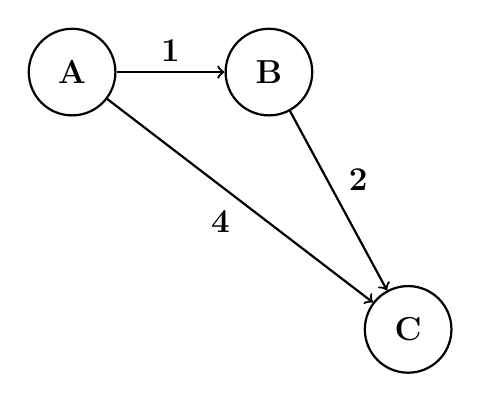
\begin{tikzpicture}[node distance=2.5cm, main node/.style={circle, draw, thick, minimum size=1.1cm, font=\large\bfseries}]
    \node[main node] (A) {A};
    \node[main node, right of=A] (B) {B};
    \node[main node, below right of=A, xshift=2.5cm, yshift=-1.5cm] (C) {C};

    \draw[->, thick] (A) -- node[above, font=\large\bfseries] {1} (B);
    \draw[->, thick] (A) -- node[below left, font=\large\bfseries] {4} (C);
    \draw[->, thick] (B) -- node[above right, font=\large\bfseries] {2} (C);
\end{tikzpicture}
\end{column}

\begin{column}{0.45\textwidth}
\textbf{Edges with costs:}
\begin{itemize}
  \item A to B: \textbf{1}
  \item A to C: \textbf{4}
  \item B to C: \textbf{2}
\end{itemize}
\end{column}
\end{columns}
\end{frame}

\begin{frame}
\frametitle{Problem Statement}
\begin{itemize}
    \item The shortest path problem seeks the path from source (A) to sink (C) with minimal total cost.
    \item Traditional algorithms: Dijkstra, Bellman-Ford.
    \item Here, we formulate it as a Linear Program (LP) using network flow.
\end{itemize}
\end{frame}

\begin{frame}
\frametitle{LP Formulation: Variables and Objective}
Variables (flow on edges):
\begin{itemize}
    \item \(x_{AB}\): flow from A to B
    \item \(x_{AC}\): flow from A to C
    \item \(x_{BC}\): flow from B to C
\end{itemize}

Objective: Minimize total cost
\[
\min \; 1 \cdot x_{AB} + 4 \cdot x_{AC} + 2 \cdot x_{BC}
\]
\end{frame}

\begin{frame}[shrink]
\frametitle{LP Formulation: Constraints}

\begin{center}
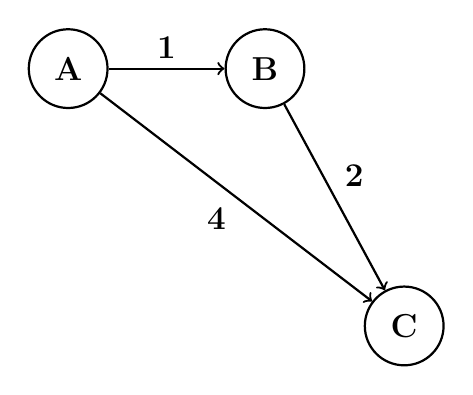
\begin{tikzpicture}[node distance=2.5cm, main node/.style={circle, draw, thick, minimum size=1.0cm, font=\large\bfseries}]
    \node[main node] (A) {A};
    \node[main node, right of=A] (B) {B};
    \node[main node, below right of=A, xshift=2.5cm, yshift=-1.5cm] (C) {C};

    \draw[->, thick] (A) -- node[above, font=\large\bfseries] {1} (B);
    \draw[->, thick] (A) -- node[below left, font=\large\bfseries] {4} (C);
    \draw[->, thick] (B) -- node[above right, font=\large\bfseries] {2} (C);
\end{tikzpicture}
\end{center}

Flow conservation (net flow out):
\begin{itemize}
  \item Source A: net out = 1 \quad \(x_{AB} + x_{AC} = 1\)
  \item Intermediate B: net out = 0 \quad \(x_{BC} - x_{AB} = 0\)
  \item Sink C: net out = -1 \quad \(-(x_{AC} + x_{BC}) = -1\) or \(x_{AC} + x_{BC} = 1\)
\end{itemize}
Non-negativity: \(x_{AB}, x_{AC}, x_{BC} \ge 0\)
\end{frame}

\begin{frame}[fragile]
\frametitle{Solving with PuLP}
\begin{lstlisting}
import pulp as pl

prob = pl.LpProblem("ShortestPath", pl.LpMinimize)

x_ab = prob.add_variable("x_ab", lowBound=0)
x_ac = prob.add_variable("x_ac", lowBound=0)
x_bc = prob.add_variable("x_bc", lowBound=0)

prob += 1*x_ab + 4*x_ac + 2*x_bc

prob += x_ab + x_ac == 1, "Node_A"
prob += x_bc - x_ab == 0, "Node_B"
prob += x_ac + x_bc == 1, "Node_C"

res = prob.solve()
\end{lstlisting}
\end{frame}



\begin{frame}
\frametitle{Optimal Solution}
\begin{itemize}
  \item \(x_{AB} = 1\)
  \item \(x_{AC} = 0\)
  \item \(x_{BC} = 1\)
  \item Total Cost = 3
\end{itemize}

Path: A \(\rightarrow\) B \(\rightarrow\) C (cost 1 + 2 = 3)
\end{frame}

\begin{frame}
\frametitle{Conclusion}
\begin{itemize}
    \item The LP formulation models the shortest path as a min-cost flow problem with unit supply/demand.
    \item Advantages: Handles variants (e.g., capacities); solvable with LP solvers.
    \item Note: For pure shortest path, integer solutions are guaranteed due to network structure.
\end{itemize}.
\end{frame}

\begin{frame}
\frametitle{Dijkstra's Algorithm: Step 1 - Initialization}
Find the shortest path from A to C.

\begin{center}
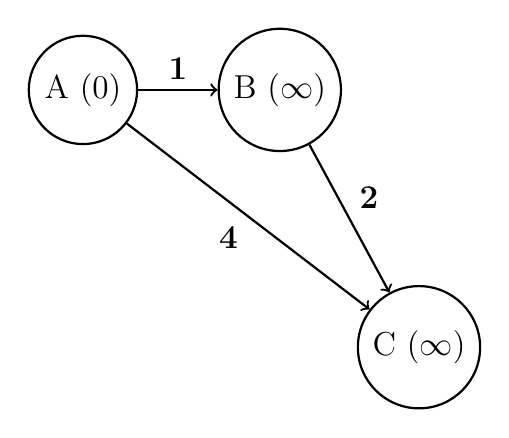
\begin{tikzpicture}[node distance=2.5cm, main node/.style={circle, draw, thick, minimum size=1.2cm, font=\large}]
    \node[main node] (A) {A (0)};
    \node[main node, right of=A] (B) {B (\(\infty\))};
    \node[main node, below right of=A, xshift=2.5cm, yshift=-1.5cm] (C) {C (\(\infty\))};

    \draw[->, thick] (A) -- node[above, font=\large\bfseries] {1} (B);
    \draw[->, thick] (A) -- node[below left, font=\large\bfseries] {4} (C);
    \draw[->, thick] (B) -- node[above right, font=\large\bfseries] {2} (C);
\end{tikzpicture}
\end{center}

- Start at node A, set distance to 0.
- Initialize distances to all other nodes as \(\infty\).
- Set A as the current node.
\end{frame}

\begin{frame}
\frametitle{Dijkstra's Algorithm: Step 2 - Update Distances}
\begin{center}
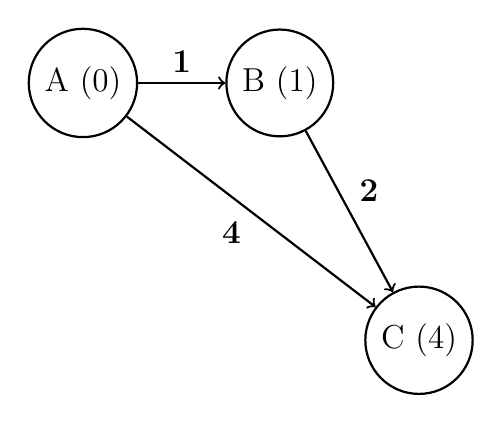
\begin{tikzpicture}[node distance=2.5cm, main node/.style={circle, draw, thick, minimum size=1.2cm, font=\large}]
    \node[main node] (A) {A (0)};
    \node[main node, right of=A] (B) {B (1)};
    \node[main node, below right of=A, xshift=2.5cm, yshift=-1.5cm] (C) {C (4)};

    \draw[->, thick] (A) -- node[above, font=\large\bfseries] {1} (B);
    \draw[->, thick] (A) -- node[below left, font=\large\bfseries] {4} (C);
    \draw[->, thick] (B) -- node[above right, font=\large\bfseries] {2} (C);
\end{tikzpicture}
\end{center}

- Update distances from A:
  - B: \(0 + 1 = 1\) (update from \(\infty\))
  - C: \(0 + 4 = 4\) (update from \(\infty\))
- Mark A as visited.
- Move to unvisited node with smallest distance: B (1).
\end{frame}

\begin{frame}
\frametitle{Dijkstra's Algorithm: Step 3 - Final Path}
\begin{center}
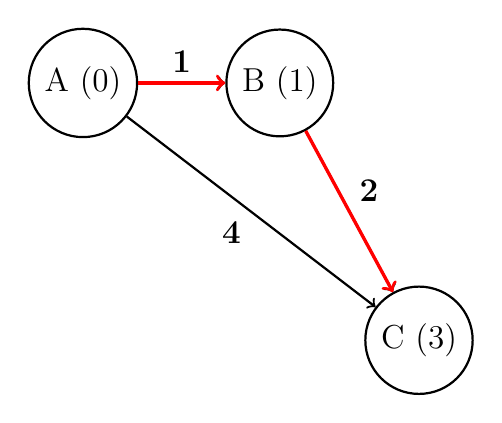
\begin{tikzpicture}[node distance=2.5cm, main node/.style={circle, draw, thick, minimum size=1.2cm, font=\large}]
    \node[main node] (A) {A (0)};
    \node[main node, right of=A] (B) {B (1)};
    \node[main node, below right of=A, xshift=2.5cm, yshift=-1.5cm] (C) {C (3)};

    \draw[->, thick] (A) -- node[above, font=\large\bfseries] {1} (B);
    \draw[->, thick] (A) -- node[below left, font=\large\bfseries] {4} (C);
    \draw[->, thick] (B) -- node[above right, font=\large\bfseries] {2} (C);
    \draw[->, very thick, red] (A) -- (B);
    \draw[->, very thick, red] (B) -- (C);
\end{tikzpicture}
\end{center}

- Update distances from B:
  - C: \(\min(4, 1 + 2) = 3\) (update from 4)
- Mark B as visited.
- Only unvisited node is C (3), mark as visited.
- Shortest path: A \(\rightarrow\) B \(\rightarrow\) C with total cost 3.
\end{frame}



\begin{frame}
  \begin{center}
    \Huge{\textbf{Sensitivity Analysis in Linear Programming}} \\[1em]
    \Large{Shadow Prices and Reduced Costs} \\[1em]
    \vspace{1cm}
    %\includegraphics[width=0.3\textwidth]{example-image} % Optional: Add an image
  \end{center}
  \begin{itemize}
    \item Using Par, Inc. Golf Bag Production as Example
  \end{itemize}
\end{frame}

\begin{frame}{Introduction to Sensitivity Analysis}
Sensitivity analysis examines how changes in LP parameters (objective coefficients, constraint RHS) affect the optimal solution.

\vspace{0.2em}
\begin{columns}[T]
\begin{column}{0.48\textwidth}
\begin{block}{Why Important?}
\small
\begin{itemize}\setlength{\itemsep}{0.2em}
  \item Tests robustness of the optimal solution
  \item Quantifies marginal value of resources
  \item Identifies critical bottlenecks
\end{itemize}
\end{block}
\end{column}

\begin{column}{0.48\textwidth}
\begin{block}{Key Concepts}
\small
\begin{itemize}\setlength{\itemsep}{0.2em}
  \item \textbf{Shadow prices / Dual variables} (constraints)
  \item \textbf{Reduced costs} (decision variables)
  \item \textbf{Ranges of validity}
\end{itemize}
\end{block}
\end{column}
\end{columns}

\vspace{0.3em}
\begin{exampleblock}{Solver Terminology: Shadow Prices = Dual Variables}
\small In Python's \texttt{PuLP} solver output, shadow prices are called \textbf{dual variables} (accessed via \texttt{c.pi}), whereas Excel Solver calls them \textbf{shadow prices}.
\end{exampleblock}
\end{frame}


\begin{frame}[shrink]
\frametitle{Recap of Par, Inc. Problem}
\textbf{Decision variables:} \\
Let \(x_s\) = number of standard golf bags produced per week,\\
\(x_d\) = number of deluxe golf bags produced per week. \\
Both \(x_s, x_d \ge 0\).

\textbf{Objective function:} \\
Maximize weekly profit:
\[
\max \; Z = 10x_s + 9x_d
\]

\textbf{Subject to capacity constraints:}
\[
\begin{aligned}
\frac{7}{10}x_s + x_d &\le 630 &\text{(Cutting \& Dyeing)} \\
\frac{1}{2}x_s + \frac{5}{6}x_d &\le 600 &\text{(Sewing)} \\
x_s + \frac{2}{3}x_d &\le 708 &\text{(Finishing)} \\
0.1x_s + 0.25x_d &\le 135 &\text{(Inspection \& Packaging)} \\
x_s, x_d &\ge 0
\end{aligned}
\]
\end{frame}



\begin{frame}{Writing the PuLP Code}
\begin{exampleblock}{Gemini Prompt}
\vspace{0.1cm}
Here is an linear program:
\(
\max \; Z = 10x_s + 9x_d
\)
s.t. 
\(\frac{7}{10}x_s + x_d\le 630; \frac{1}{2}x_s + \frac{5}{6}x_d; x_s + \frac{2}{3}x_d\le 708; 0.1x_s + 0.25x_d\le 135; 
x_s, x_d \ge 0\). Write me a python code that solves the linear program using PuLP. Also add code that will compute \textbf{reduced costs}, \textbf{shadow prices}, and \textbf{indicate which constraints are loose or tight}. 
\vspace{0.1cm}
\end{exampleblock}
\end{frame}


\begin{frame}[fragile]
\frametitle{PuLP Code with Shadow Prices and Reduced Costs}
\begin{lstlisting}
import pulp as pl

# Model
prob = pl.LpProblem("Par_Inc_Golf_Bags", pl.LpMaximize)

# Variables (continuous  0; add cat='Integer' if you ever need integrality)
x_s = prob.add_variable("Standard_Bags", lowBound=0)
x_d = prob.add_variable("Deluxe_Bags",   lowBound=0)

# Objective
prob += 10 * x_s + 9 * x_d, "Maximize_Profit"

# Constraints
prob += 0.7 * x_s + 1.0   * x_d <= 630, "Cutting_Dyeing"
prob += 0.5 * x_s + (5/6) * x_d <= 600, "Sewing"
prob += 1.0 * x_s + (2/3) * x_d <= 708, "Finishing"
prob += 0.1 * x_s + 0.25  * x_d <= 135, "Inspection_Packaging"

# Solve with CBC so reduced costs are available
res = prob.solve()
\end{lstlisting}
\end{frame}

\begin{frame}[fragile]
\frametitle{PuLP Code with Shadow Prices and Reduced Costs}
\begin{lstlisting}[basicstyle=\ttfamily\scriptsize]
# Report primal solution
print("Status:", res.status.name)
print(f"Standard Bags  = {x_s.varValue:,.2f}")
print(f"Deluxe Bags    = {x_d.varValue:,.2f}")
print(f"Maximum Profit = ${pl.value(prob.objective):,.2f}")

# Shadow Prices (called Dual Variables in PuLP) and Slacks
print("\nSensitivity Analysis -- Constraints:")
for c in prob.constraints():
    shadow_price = abs(c.pi) if c.pi is not None else 0.0
    slack = abs(c.slack) if c.slack is not None else 0.0
    print(f"  {c.name:<22}: Shadow Price = ${shadow_price:.4f}, Slack = {slack:.2f} hrs")

# Reduced Costs
print("\nSensitivity Analysis -- Decision Variables:")
for v in prob.variables():
    print(f"  {v.name:<15}: Value = {v.varValue:,.2f}, Reduced Cost = ${v.dj:.4f}")
\end{lstlisting}
\end{frame}

% ==============================================================================
% SLIDE: Obtaining Shadow Prices in Excel Solver
% ==============================================================================
\begin{frame}{Obtaining Shadow Prices in Excel Solver}
\begin{columns}[T]
\begin{column}{0.48\textwidth}
\begin{block}{Step-by-Step in Excel Solver}
\footnotesize
\begin{enumerate}\setlength{\itemsep}{0.1em}
  \item \textbf{Set Up Model:} Enter objective, variables, and constraints in \textbf{Data $\rightarrow$ Solver}.
  \item \textbf{Choose Method:} Select \textbf{Simplex LP} (required for sensitivity output).
  \item \textbf{Select Report:} Click \textbf{Solve}, then highlight \textbf{Sensitivity} under \textbf{Reports}.
  \item \textbf{Generate Tab:} Click \textbf{OK} to create the \textbf{Sensitivity Report} tab.
\end{enumerate}
\end{block}
\end{column}

\begin{column}{0.48\textwidth}
\begin{block}{Reading the Sensitivity Report}
\footnotesize
\begin{itemize}\setlength{\itemsep}{0.2em}
  \item \textbf{Variable Cells Table (Top):} Reports \textbf{Final Value} ($x_j^*$), \textbf{Reduced Cost} ($d_j$), and allowable objective ranges.
  \item \textbf{Constraints Table (Bottom):} Reports \textbf{Final Value} (used hrs), \textbf{Shadow Price} ($\pi_i$), and allowable RHS ranges.
\end{itemize}
\end{block}
\end{column}
\end{columns}

\vspace{0.1em}
\begin{exampleblock}{Excel Solver vs.\ Python \texttt{PuLP} Terminology}
\footnotesize
\textbf{Shadow Prices = Dual Variables:} Excel labels marginal constraint values \textbf{Shadow Price} (Constraints table), whereas Python's \texttt{PuLP} calls them \textbf{Dual Variables} (\texttt{c.pi}). Both tools use \textbf{Reduced Cost} (\texttt{v.dj}).
\end{exampleblock}
\end{frame}


% --- Slide 1: Primal Solution and Binding Constraints ---
\begin{frame}{Optimal Solution}
No need to read the code. Just run it to get this:
    \begin{columns}
        \column{0.5\textwidth}
        \centering
        \begin{block}{Optimal Production Plan}
            \vspace{0.2cm}
            \begin{itemize}
                \item \textbf{Standard Bags} (\(x_s\)): 540
                \item \textbf{Deluxe Bags} (\(x_d\)): 252
            \end{itemize}
            \vspace{0.2cm}
        \end{block}

        \begin{alertblock}{Maximum Profit}
            \centering
            \textbf{\Large \(\$7,668.00\)}
        \end{alertblock}
        
        \column{0.5\textwidth}
        \centering
        \begin{alertblock}{Binding Constraints}
            \vspace{0.2cm}
            These resources are fully utilized (\(\text{Slack} = 0\)) and define the optimal solution.
            \vspace{0.1cm}
            \begin{itemize}
                \item \textbf{Cutting/Dyeing} (\(\mathbf{C_1}\)): \(0.7 x_s + 1.0 x_d \le 630\)
                \item \textbf{Finishing} (\(\mathbf{C_3}\)): \(1.0 x_s + \frac{2}{3} x_d \le 708\)
            \end{itemize}
            \vspace{0.2cm}
        \end{alertblock}
    \end{columns}

\end{frame}

% ==============================================================================
% SLIDE 1: What Is an Extra Hour Worth? (Shadow Price)
% ==============================================================================
\begin{frame}{What Is an Extra Hour Worth? (Shadow Price)}
\begin{block}{Definition: Shadow Price (also called Dual Variable)}
\small
\setlength{\abovedisplayskip}{4pt}\setlength{\belowdisplayskip}{4pt}
The marginal change in optimal profit per 1-unit increase in resource capacity (RHS):
\[
\text{Shadow Price / Dual Variable } (\pi_i) = \frac{\Delta \text{Optimal Profit}}{\Delta \text{Resource Capacity } (b_i)}
\]

\footnotesize \textbf{Terminology:} Excel calls $\pi_i$ a \textbf{shadow price}; Python's \texttt{PuLP} calls it a \textbf{dual variable} (\texttt{c.pi}).\par
\end{block}

\vspace{0.1em}
\begin{columns}[T]
\begin{column}{0.48\textwidth}
\begin{block}{Managerial Willingness to Pay}
\small
\begin{itemize}\setlength{\itemsep}{0.15em}
  \item \textbf{Upper Limit:} Max premium worth paying for extra bottleneck capacity.
  \item \textbf{Overtime Limit:} Paying up to \textbf{\$4.38/hr} in Cutting overtime is profitable.
\end{itemize}
\end{block}
\end{column}

\begin{column}{0.48\textwidth}
\begin{alertblock}{The Golden Rule of Slack}
\small
\begin{itemize}\setlength{\itemsep}{0.15em}
  \item If $\mathbf{\text{Slack} > 0}$, then $\mathbf{\text{Shadow Price} = \$0.00}$.
  \item \textbf{Intuition:} Why pay for extra hours when surplus capacity is already idle?
\end{itemize}
\end{alertblock}
\end{column}
\end{columns}
\end{frame}

% ==============================================================================
% SLIDE 2: Par, Inc. Shadow Prices: Where Is the Bottleneck?
% ==============================================================================
\begin{frame}{Par, Inc. Shadow Prices: Where Is the Bottleneck?}
\begin{table}[h]
\centering
\footnotesize
\renewcommand{\arraystretch}{1.15}
\setlength{\tabcolsep}{4pt}
\begin{tabular}{lccccc}
\hline
\textbf{Department} & \textbf{Available} & \textbf{Used} & \textbf{Slack} & \textbf{Shadow Price} & \textbf{Status} \\
\hline
Cutting \& Dyeing   & 630 hr & 630 hr & 0 hr   & \$4.375 / hr  & \alert{\textbf{Bottleneck}} \\
Sewing              & 600 hr & 480 hr & 120 hr & \$0.000 / hr  & Surplus \\
Finishing           & 708 hr & 708 hr & 0 hr   & \$6.938 / hr  & \alert{\textbf{Top Bottleneck}} \\
Inspection \& Pkg   & 135 hr & 117 hr & 18 hr  & \$0.000 / hr  & Surplus \\
\hline
\end{tabular}
\end{table}

\vspace{-0.3em}
\begin{columns}[T]
\begin{column}{0.48\textwidth}
\begin{alertblock}{Bottleneck Resources (Slack = 0)}
\small
\begin{itemize}\setlength{\itemsep}{0.2em}
  \item \textbf{Finishing (\$6.94/hr):} Most critical; highest priority for overtime/expansion.
  \item \textbf{Cutting \& Dyeing (\$4.38/hr):} Second bottleneck; each extra hour yields \$4.38.
\end{itemize}
\end{alertblock}
\end{column}

\begin{column}{0.48\textwidth}
\begin{exampleblock}{Surplus Resources ($\text{Slack} > 0$)}
\small
\begin{itemize}\setlength{\itemsep}{0.2em}
  \item \textbf{Sewing (120 idle hrs)} and \textbf{Inspection (18 idle hrs)}.
  \item Extra capacity generates \textbf{\$0.00} profit because resources exceed demand.
\end{itemize}
\end{exampleblock}
\end{column}
\end{columns}
\end{frame}

% ==============================================================================
% SLIDE 3: The "Standard Plus" Bag: Pricing Out Resources
% ==============================================================================
\begin{frame}{The ``Standard Plus'' Bag: Pricing Out Resources}
\begin{block}{Marketing Proposal: New ``Standard Plus'' Model}
\small
Requires: 0.80 hr Cutting, 0.60 hr Sewing, 0.80 hr Finishing, and 0.15 hr Inspection.
\end{block}

\vspace{-0.3em}
\begin{columns}[T]
\begin{column}{0.53\textwidth}
\centering
\scriptsize
\setlength{\tabcolsep}{2.5pt}
\begin{tabular}{lccc}
\hline
\textbf{Dept.} & \textbf{Hours} & \textbf{Shadow Price} & \textbf{Opp. Cost} \\
\hline
Cutting    & 0.80 & $\times\ \$4.375$ & $\$3.50$ \\
Sewing     & 0.60 & $\times\ \$0.000$ & $\$0.00$ \\
Finishing  & 0.80 & $\times\ \$6.938$ & $\$5.55$ \\
Inspection & 0.15 & $\times\ \$0.000$ & $\$0.00$ \\
\hline
\multicolumn{3}{l}{\textbf{Hurdle Rate ($\sum a_{ij}\pi_i$):}} & \alert{\textbf{\$9.05 / bag}} \\
\hline
\end{tabular}

\vspace{0.4em}
\scriptsize{\textit{Surplus departments contribute \$0.00!}}
\end{column}

\begin{column}{0.44\textwidth}
\begin{alertblock}{Key Economic Insight}
\small
\begin{itemize}\setlength{\itemsep}{0.2em}
  \item Hurdle rate: \alert{\textbf{\$9.05 / bag}}.
  \item Diverting bottleneck hours \textbf{destroys \$9.05} profit.
  \item Viable only if unit profit $> \$9.05$.
\end{itemize}
\end{alertblock}
\end{column}
\end{columns}
\end{frame}

% ==============================================================================
% SLIDE 4: The Strategic Payoff: Fast Decisions Without Re-Solving
% ==============================================================================
\begin{frame}{The Strategic Payoff: Evaluating the Net Margin}
\begin{block}{Net Economic Margin: $\text{Unit Profit} - \$9.05\text{ Hurdle Rate}$}
\small
Compare proposed unit profit against the $\$9.05$ opportunity cost of diverted bottleneck capacity:
\end{block}

\vspace{-0.1em}
\begin{columns}[T]
\begin{column}{0.48\textwidth}
\begin{exampleblock}{Scenario A: Profit = \$10.00 / bag}
\small
{\footnotesize\setlength{\abovedisplayskip}{4pt}\setlength{\belowdisplayskip}{4pt}
\[ \text{Margin} = \$10.00 - \$9.05 = \mathbf{+\$0.95 > 0} \]}
\textbf{Decision: PRODUCE!}
\begin{itemize}\setlength{\itemsep}{0.1em}
  \item Clears resource hurdle rate.
  \item Increases total company profit.
\end{itemize}
\end{exampleblock}
\end{column}

\begin{column}{0.48\textwidth}
\begin{alertblock}{Scenario B: Profit = \$8.50 / bag}
\small
{\footnotesize\setlength{\abovedisplayskip}{4pt}\setlength{\belowdisplayskip}{4pt}
\[ \text{Margin} = \$8.50 - \$9.05 = \mathbf{-\$0.55 < 0} \]}
\textbf{Decision: REJECT!}
\begin{itemize}\setlength{\itemsep}{0.1em}
  \item Fails resource hurdle rate.
  \item Destroys \textbf{\$0.55} profit per bag.
\end{itemize}
\end{alertblock}
\end{column}
\end{columns}

\vspace{0.2em}
\centering \footnotesize \textbf{Bridge to Theory:} In Linear Programming, this exact net margin ($\text{Unit Profit} - \text{Opportunity Cost}$) is called the \alert{\textbf{Reduced Cost}}!
\end{frame}

% ==============================================================================
% SLIDE 5: Formalizing Reduced Cost at Optimality
% ==============================================================================
\begin{frame}{Formalizing Reduced Cost ($d_j$) at Optimality}
\begin{block}{Definition: Reduced Cost as Net Resource Margin}
\small
\setlength{\abovedisplayskip}{3pt}\setlength{\belowdisplayskip}{3pt}
Net margin per unit: unit profit minus the shadow value of scarce resources consumed:
\[
\text{Reduced Cost } (d_j) = \underbrace{\text{Unit Profit } (c_j)}_{\text{Revenue Earned}} - \underbrace{\sum_{i=1}^m a_{ij} \pi_i}_{\text{Opportunity Cost of Resources}}
\]
\end{block}

\vspace{-0.1em}
\begin{columns}[T]
\begin{column}{0.48\textwidth}
\begin{exampleblock}{Produced Items ($x_j^* > 0 \implies d_j = \$0.00$)}
\small
\begin{itemize}\setlength{\itemsep}{0.15em}
  \item \textbf{Reduced Cost = \$0.00} (Standard \& Deluxe).
  \item \textbf{Why?} At optimality, unit profit equals opportunity cost ($c_j = \sum_i a_{ij}\pi_i$).
\end{itemize}
\end{exampleblock}
\end{column}

\begin{column}{0.48\textwidth}
\begin{alertblock}{Unproduced Items ($x_j^* = 0 \implies d_j \le \$0.00$)}
\small
\begin{itemize}\setlength{\itemsep}{0.15em}
  \item \textbf{Reduced Cost $\le \$0.00$} (Scenario B: $-\$0.55$).
  \item \textbf{Why?} Resource cost exceeds profit; $|d_j|$ is the profit shortfall per unit.
\end{itemize}
\end{alertblock}
\end{column}
\end{columns}
\end{frame}

% ==============================================================================
% SLIDE 6: Alternative Approach: Reformulating & Re-Solving the LP
% ==============================================================================
\begin{frame}{Alternative Approach: Reformulating the LP}{Adding the ``Standard Plus'' Bag ($x_p$) as a Third Decision Variable}
\begin{block}{Expanded 3-Product Formulation}
\small
Let $x_p \ge 0$ denote weekly production of the new \textbf{Standard Plus} bag with unit profit $c_p \in \{\$10.00, \$8.50\}$:
\[
\max \; Z = 10x_s + 9x_d + \alert{\mathbf{c_p x_p}}
\]
\vspace{-0.8em}
\[
\begin{aligned}
0.7x_s + 1.0x_d + \alert{\mathbf{0.80x_p}} &\le 630 &&\text{(Cutting \& Dyeing)} \\
0.5x_s + \tfrac{5}{6}x_d + \alert{\mathbf{0.60x_p}} &\le 600 &&\text{(Sewing)} \\
1.0x_s + \tfrac{2}{3}x_d + \alert{\mathbf{0.80x_p}} &\le 708 &&\text{(Finishing)} \\
0.1x_s + 0.25x_d + \alert{\mathbf{0.15x_p}} &\le 135 &&\text{(Inspection \& Packaging)} \\
x_s,\; x_d,\; \alert{\mathbf{x_p}} &\ge 0
\end{aligned}
\]
\end{block}
\end{frame}

% ==============================================================================
% SLIDE 7: Re-Solved LP Results vs. Shadow Price Shortcuts
% ==============================================================================
\begin{frame}{Re-Solving the Expanded LP: Exact Confirmation}
\begin{columns}[T]
\begin{column}{0.48\textwidth}
\begin{exampleblock}{Scenario A: $c_p = \$10.00$ ($d_p = +\$0.95$)}
\small
\begin{itemize}\setlength{\itemsep}{0.2em}
  \item \textbf{Optimal Mix:} $x_s^* = 260$, $x_d^* = 0$, $\alert{\mathbf{x_p^* = 560}}$
  \item \textbf{New Profit:} $\mathbf{Z^* = \$8,200.00}$ ($+\$532$ gain)
  \item \textbf{New Reduced Costs:} $d_s = \$0$, $d_p = \$0$ (produced); $d_d = -\$2.11$ (Deluxe priced out!)
\end{itemize}
\end{exampleblock}
\end{column}

\begin{column}{0.48\textwidth}
\begin{alertblock}{Scenario B: $c_p = \$8.50$ ($d_p = -\$0.55$)}
\small
\begin{itemize}\setlength{\itemsep}{0.2em}
  \item \textbf{Optimal Mix:} $x_s^* = 540$, $x_d^* = 252$, $\alert{\mathbf{x_p^* = 0}}$
  \item \textbf{New Profit:} $\mathbf{Z^* = \$7,668.00}$ (unchanged)
  \item \textbf{Reduced Costs:} $d_s = \$0$, $d_d = \$0$ (produced); $\alert{\mathbf{d_p = -\$0.55}}$ (exact match!)
\end{itemize}
\end{alertblock}
\end{column}
\end{columns}

\vspace{0.2em}
\begin{block}{Why Both Perspectives Matter}
\footnotesize
\textbf{Shadow pricing} tells us \textit{instantly} whether $x_p^* > 0$ ($c_p > \$9.05$); \textbf{re-solving the LP} is needed only when $c_p > \$9.05$ to find the exact new production quantities $(260, 0, 560)$.
\end{block}
\end{frame}

% ==============================================================================
% SLIDE 10: CASE STUDY: PARKET SISTERS PENCIL & PEN FACTORY
% ==============================================================================
\begin{frame}{Case Study: Parket Sisters Pencil \& Pen Factory}{Multi-Product, Multi-Material Production Optimization}
    \begin{columns}[T]
        \begin{column}{0.46\textwidth}
            \begin{block}{Products \& Profit Margins}
                \begin{itemize}\setlength{\itemsep}{0.2em}
                    \item $X_1$: \textbf{Ballpoint Pens} (\$3.00 profit)
                    \item $X_2$: \textbf{Mechanical Pencils} (\$3.00 profit)
                    \item $X_3$: \textbf{Fountain Pens} (\$5.00 profit)
                \end{itemize}
            \end{block}
            \begin{block}{Material Inventory Limits}
                \begin{itemize}\setlength{\itemsep}{0.2em}
                    \item \textbf{Plastic:} 1,000 oz available
                    \item \textbf{Chrome:} 1,200 oz available
                    \item \textbf{Stainless Steel:} 2,000 oz available
                \end{itemize}
            \end{block}
        \end{column}
        \begin{column}{0.52\textwidth}
            \begin{exampleblock}{Linear Programming Model}
                \footnotesize
                \[ \text{Maximize } Z = 3.0 X_1 + 3.0 X_2 + 5.0 X_3 \]
                \textbf{Subject to:}
                \begin{align*}
                \text{Plastic:}\quad  & 1.2 X_1 + 1.7 X_2 + 1.2 X_3 \le 1000 \\
                \text{Chrome:}\quad   & 0.8 X_1 + 0.0 X_2 + 2.3 X_3 \le 1200 \\
                \text{Steel:}\quad    & 2.0 X_1 + 3.0 X_2 + 4.5 X_3 \le 2000 \\
                & X_1, X_2, X_3 \ge 0
                \end{align*}
            \end{exampleblock}
            \vspace{-0.3em}
            \begin{alertblock}{Decisions Ahead}
                \scriptsize Extra steel offer, supply cut, and R\&D redesign.
            \end{alertblock}
        \end{column}
    \end{columns}
\end{frame}

% ==============================================================================
% SLIDE 11: PARKET SISTERS: PULP OPTIMIZATION DASHBOARD
% ==============================================================================
\begin{frame}{Parket Sisters: PuLP Optimization Dashboard}{Baseline Primal Production Plan and Dual Resource Audit}
    \begin{block}{Primal Production Plan (Optimal Objective: $Z^* = \$2,766.67$)}
        \centering
        \footnotesize
        \setlength{\tabcolsep}{4pt}
        \begin{tabular}{lcccc}
            \hline
            \textbf{Product} & \textbf{Quantity ($X_j^*$)} & \textbf{Profit} & \textbf{Reduced Cost} & \textbf{Status} \\
            \hline
            $X_1$ (Ballpoint)    & 700.00 units  & \$3.00 & \$0.0000  & \alert{\textbf{In Production}} \\
            $X_2$ (Mech. Pencil) & 0.00 units    & \$3.00 & -\$1.3833 & \textbf{Excluded} \\
            $X_3$ (Fountain Pen) & 133.33 units  & \$5.00 & \$0.0000  & \alert{\textbf{In Production}} \\
            \hline
        \end{tabular}
    \end{block}
    \vspace{0.1em}
    \begin{exampleblock}{Dual Resource Values \& Capacity Utilization}
        \centering
        \footnotesize
        \setlength{\tabcolsep}{4pt}
        \begin{tabular}{lccccc}
            \hline
            \textbf{Material} & \textbf{Available} & \textbf{Used} & \textbf{Slack} & \textbf{Shadow Price} & \textbf{Status} \\
            \hline
            Plastic          & 1,000 oz & 1,000 oz & 0 oz   & \$1.1667 / oz & \alert{\textbf{Bottleneck}} \\
            Chrome           & 1,200 oz & 866.7 oz & 333.3 oz & \$0.0000 / oz & Surplus \\
            Stainless Steel  & 2,000 oz & 2,000 oz & 0 oz   & \$0.8000 / oz & \alert{\textbf{Bottleneck}} \\
            \hline
        \end{tabular}
    \end{exampleblock}
\end{frame}

% ==============================================================================
% SLIDE 12: CASE DECISION 1: SUPPLIER OFFER FOR EXTRA STAINLESS STEEL
% ==============================================================================
\begin{frame}{Decision 1: Supplier Offer for Extra Steel}{Capitalizing on Bottleneck Capacity Expansion}
    \begin{block}{The Supplier's Offer}
        \small
        A distributor offers an additional \textbf{500 oz of Stainless Steel} at a \textbf{\$0.60/oz premium} above standard contract price.
    \end{block}
    \vspace{-0.2em}
    \begin{columns}[T]
        \begin{column}{0.48\textwidth}
            \begin{block}{3-Step Evaluation}
                \textbf{1. Range of Feasibility:}
                \begin{itemize}\setlength{\itemsep}{0.1em}
                    \item Allowable increase: 555.56 oz.
                    \item $500 \le 555.56 \implies \mathbf{\pi_{\text{steel}} = \$0.80}$.
                \end{itemize}
                \vspace{0.2em}
                \textbf{2. Marginal Spread:}
                \begin{itemize}\setlength{\itemsep}{0.1em}
                    \item Value: \textbf{\$0.80/oz} vs. Cost: \textbf{\$0.60/oz}
                    \item Net Spread: $\mathbf{+\$0.20 / \text{oz}}$
                \end{itemize}
            \end{block}
        \end{column}
        \begin{column}{0.48\textwidth}
            \begin{exampleblock}{3. Total Net Profit Impact}
                \small
                \begin{align*}
                \Delta \text{Gross} &= 500 \times \$0.80 = +\$400.00 \\
                \text{Cost}         &= 500 \times \$0.60 = -\$300.00 \\
                \mathbf{\Delta \text{Net}} &= \mathbf{+\$100.00}
                \end{align*}
            \end{exampleblock}
            \vspace{-0.2em}
            \begin{alertblock}{Managerial Decision}
                \centering \small
                \textbf{ACCEPT THE OFFER!}\\
                Net company profit increases by \textbf{+\$100.00}.
            \end{alertblock}
        \end{column}
    \end{columns}
\end{frame}

% ==============================================================================
% SLIDE 12B: DECISION 1 VIA LP RE-OPTIMIZATION
% ==============================================================================
\begin{frame}{Decision 1: Re-Solving the Modified LP}{Without Allowable-Increase Tables, We Simply Update the RHS!}
    \begin{columns}[T]
        \begin{column}{0.52\textwidth}
            \begin{block}{Modified LP (Steel RHS $= 2,500\text{ oz}$)}
                \footnotesize
                \[ \max \; Z = 3.0 X_1 + 3.0 X_2 + 5.0 X_3 - \alert{\mathbf{300}} \]
                \vspace{-0.6em}
                \begin{align*}
                \text{Plastic:}\quad & 1.2 X_1 + 1.7 X_2 + 1.2 X_3 \le 1000 \\
                \text{Chrome:}\quad  & 0.8 X_1 + 0.0 X_2 + 2.3 X_3 \le 1200 \\
                \text{Steel:}\quad   & 2.0 X_1 + 3.0 X_2 + 4.5 X_3 \le \alert{\mathbf{2500}} \\
                & X_1,\; X_2,\; X_3 \ge 0
                \end{align*}
            \end{block}
        \end{column}
        \begin{column}{0.45\textwidth}
            \begin{exampleblock}{Re-Solved Optimal Solution}
                \footnotesize
                \begin{itemize}\setlength{\itemsep}{0.2em}
                    \item $X_1^* = 500.00$ Ballpoint Pens
                    \item $X_2^* = 0.00$ Mech. Pencils
                    \item $X_3^* = 333.33$ Fountain Pens
                    \item \textbf{Gross Profit:} $\$3,166.67$ ($+\$400$)
                    \item \textbf{Less Steel Premium:} $-\$300.00$
                    \item \textbf{Net Profit:} $\alert{\mathbf{\$2,866.67}}$ ($\mathbf{+\$100}$)
                \end{itemize}
            \end{exampleblock}
        \end{column}
    \end{columns}
    \vspace{0.2em}
    \centering \scriptsize \textit{Re-solving confirms that all 500 extra oz of Steel are profitably absorbed without hitting the Chrome limit!}
\end{frame}

% ==============================================================================
% SLIDE 13: CASE DECISION 2: SUPPLIER DISRUPTION & CHROME SHORTAGE
% ==============================================================================
\begin{frame}{Decision 2: Supplier Disruption \& Chrome Shortage}{Assessing Supply Chain Shocks Using Slack Buffers}
    \begin{block}{Disruption Scenario}
        \small
        A logistics delay cuts Chrome supply from \textbf{1,200 oz down to 1,000 oz} (a 200 oz reduction). Should management panic?
    \end{block}
    \vspace{-0.2em}
    \begin{columns}[T]
        \begin{column}{0.48\textwidth}
            \begin{block}{Slack Buffer Analysis}
                \begin{itemize}\setlength{\itemsep}{0.1em}
                    \item \textbf{Optimal Usage:} 866.67 oz
                    \item \textbf{Available Slack:} $\mathbf{333.33\text{ oz}}$
                    \item \textbf{Disruption:} $200\text{ oz} \le 333.33\text{ oz}$
                    \item Non-binding $\implies \mathbf{\pi_{\text{chrome}} = \$0.00}$
                \end{itemize}
            \end{block}
        \end{column}
        \begin{column}{0.48\textwidth}
            \begin{exampleblock}{Impact on Operations}
                \begin{itemize}\setlength{\itemsep}{0.1em}
                    \item \textbf{Profit Impact:} $\Delta Z^* = \mathbf{\$0.00}$
                    \item \textbf{Production Mix:} $(700, 133.3)$ preserved
                    \item \textbf{Remaining Slack:} $\mathbf{133.33\text{ oz}}$
                \end{itemize}
            \end{exampleblock}
            \vspace{-0.2em}
            \begin{alertblock}{Decision: DO NOT PANIC!}
                \centering \small Buffer absorbs 100\% of shock with zero loss.
            \end{alertblock}
        \end{column}
    \end{columns}
\end{frame}

% ==============================================================================
% SLIDE 13B: DECISION 2 VIA LP RE-OPTIMIZATION
% ==============================================================================
\begin{frame}{Decision 2: Re-Solving When Chrome Supply Drops}{What If We Just Change the Chrome RHS to $1,000\text{ oz}$?}
    \begin{columns}[T]
        \begin{column}{0.52\textwidth}
            \begin{block}{Modified LP (Chrome RHS $= 1,000\text{ oz}$)}
                \footnotesize
                \[ \max \; Z = 3.0 X_1 + 3.0 X_2 + 5.0 X_3 \]
                \vspace{-0.6em}
                \begin{align*}
                \text{Plastic:}\quad & 1.2 X_1 + 1.7 X_2 + 1.2 X_3 \le 1000 \\
                \text{Chrome:}\quad  & 0.8 X_1 + 0.0 X_2 + 2.3 X_3 \le \alert{\mathbf{1000}} \\
                \text{Steel:}\quad   & 2.0 X_1 + 3.0 X_2 + 4.5 X_3 \le 2000 \\
                & X_1,\; X_2,\; X_3 \ge 0
                \end{align*}
            \end{block}
        \end{column}
        \begin{column}{0.45\textwidth}
            \begin{exampleblock}{Re-Solved Optimal Solution}
                \footnotesize
                \begin{itemize}\setlength{\itemsep}{0.2em}
                    \item $X_1^* = 700.00$, $X_2^* = 0.00$, $X_3^* = 133.33$
                    \item \textbf{Optimal Profit:} $\mathbf{Z^* = \$2,766.67}$ ($\Delta Z^* = \$0$)
                    \item \textbf{Chrome Used:} $866.67\text{ oz} \le 1,000\text{ oz}$
                    \item \textbf{New Chrome Slack:} $133.33\text{ oz}$
                \end{itemize}
            \end{exampleblock}
        \end{column}
    \end{columns}
    \vspace{0.2em}
    \centering \scriptsize \textit{Note: If the cut exceeded $333.33\text{ oz}$ (e.g., Chrome $\le 800\text{ oz}$), Chrome would become a binding bottleneck and we would HAVE to re-solve the LP!}
\end{frame}

% ==============================================================================
% SLIDE 14: CASE DECISION 3: R&D REDESIGN OF MECHANICAL PENCIL
% ==============================================================================
\begin{frame}{Decision 3: R\&D Redesign of Mechanical Pencil}{Pricing Out a Product Redesign Using Shadow Prices}
    \begin{block}{R\&D Engineering Redesign Proposal}
        \small
        Original pencil is unprofitable ($d_2 = -\$1.38$). Redesigned pencil: profit remains \textbf{\$3.00}, but consumes \textbf{1.1 oz Plastic}, \textbf{2.0 oz Chrome}, and \textbf{2.0 oz Stainless Steel}.
    \end{block}
    \vspace{-0.2em}
    \begin{columns}[T]
        \begin{column}{0.53\textwidth}
            \begin{table}[h]
                \centering
                \scriptsize
                \setlength{\tabcolsep}{2.5pt}
                \begin{tabular}{lccc}
                    \hline
                    \textbf{Material} & \textbf{Usage} & \textbf{Shadow Price} & \textbf{Opp. Cost} \\
                    \hline
                    Plastic         & 1.1 oz & $\times\ \$1.1667$ & \$1.2833 \\
                    Chrome          & 2.0 oz & $\times\ \$0.0000$ & \$0.0000 \\
                    Stainless Steel & 2.0 oz & $\times\ \$0.8000$ & \$1.6000 \\
                    \hline
                    \multicolumn{3}{l}{\textbf{Total Hurdle Rate ($\sum a_{ij}\pi_i$):}} & \alert{\textbf{\$2.8833}} \\
                    \hline
                \end{tabular}
            \end{table}
            \vspace{-0.5em}
            \scriptsize{\textit{Surplus Chrome adds \$0.00 to opportunity cost!}}
        \end{column}
        \begin{column}{0.44\textwidth}
            \begin{exampleblock}{Hurdle Rate Evaluation}
                \small
                \[ d_2^{\text{new}} = \$3.00 - \$2.88 = \mathbf{+\$0.12 > 0} \]
            \end{exampleblock}
            \vspace{-0.2em}
            \begin{alertblock}{Managerial Decision}
                \centering \small
                \textbf{APPROVE REDESIGN FOR PRODUCTION!}\\
                Clears hurdle rate; increases company profit.
            \end{alertblock}
        \end{column}
    \end{columns}
\end{frame}

% ==============================================================================
% SLIDE 14B: DECISION 3 VIA LP RE-OPTIMIZATION
% ==============================================================================
\begin{frame}{Decision 3: Re-Solving the LP with the Redesigned Pencil}{Updating the $X_2$ Technical Coefficients to Find the New Optimal Mix}
    \begin{columns}[T]
        \begin{column}{0.52\textwidth}
            \begin{block}{Modified LP (Updated $X_2$ Column)}
                \footnotesize
                \[ \max \; Z = 3.0 X_1 + \alert{\mathbf{3.0 X_2}} + 5.0 X_3 \]
                \vspace{-0.6em}
                \begin{align*}
                \text{Plastic:}\quad & 1.2 X_1 + \alert{\mathbf{1.1 X_2}} + 1.2 X_3 \le 1000 \\
                \text{Chrome:}\quad  & 0.8 X_1 + \alert{\mathbf{2.0 X_2}} + 2.3 X_3 \le 1200 \\
                \text{Steel:}\quad   & 2.0 X_1 + \alert{\mathbf{2.0 X_2}} + 4.5 X_3 \le 2000 \\
                & X_1,\; X_2,\; X_3 \ge 0
                \end{align*}
            \end{block}
        \end{column}
        \begin{column}{0.45\textwidth}
            \begin{exampleblock}{New Optimal Production Plan}
                \footnotesize
                \begin{itemize}\setlength{\itemsep}{0.15em}
                    \item $X_1^* = 457.14$ Ballpoint Pens
                    \item $\alert{\mathbf{X_2^* = 285.71}}$ \textbf{Mech. Pencils}
                    \item $X_3^* = 114.29$ Fountain Pens
                    \item \textbf{New Profit:} $\alert{\mathbf{Z^* = \$2,800.00}}$ ($+\$33.33$)
                    \item \textbf{All 3 Materials Binding!} ($\text{Slack} = 0$)
                \end{itemize}
            \end{exampleblock}
        \end{column}
    \end{columns}
    \vspace{0.2em}
    \begin{alertblock}{Why Re-Solving Is Essential Here}
        \scriptsize
        Shadow pricing told us $d_2^{\text{new}} = +\$0.12 > 0$ per pencil, so launching $X_2$ is profitable. Re-solving the LP reveals that at $X_2^* = 285.71\text{ units}$, the redesigned pencil consumes all remaining Chrome slack ($285.71 \times \$0.1167 = +\$33.33$ total profit gain)!
    \end{alertblock}
\end{frame}

% ==============================================================================
% SLIDE 15: EXECUTIVE SUMMARY: THE MANAGER'S SENSITIVITY DECISION MATRIX
% ==============================================================================
\begin{frame}{Executive Summary: Sensitivity Decision Matrix}{A 4-Quadrant Framework for Operational Decision-Making}
    \begin{columns}[T]
        \begin{column}{0.48\textwidth}
            \begin{alertblock}{1. Expanding Bottlenecks ($\pi_i > 0$)}
                \scriptsize
                \begin{itemize}\setlength{\itemsep}{0.1em}
                    \item \textbf{Action:} Authorize overtime or supplier buy.
                    \item \textbf{Pricing Rule:} Max price = Shadow Price ($\pi_i$).
                    \item \textbf{Limit:} Valid up to Allowable Increase.
                \end{itemize}
            \end{alertblock}
            \vspace{0.1em}
            \begin{block}{2. Surplus Resources ($\text{Slack}_i > 0$)}
                \scriptsize
                \begin{itemize}\setlength{\itemsep}{0.1em}
                    \item \textbf{Action:} Never pay premiums for idle assets.
                    \item \textbf{Pricing Rule:} Shadow price is strictly \textbf{\$0.00}.
                    \item \textbf{Disruptions:} Absorbed free within slack.
                \end{itemize}
            \end{block}
        \end{column}
        \begin{column}{0.48\textwidth}
            \begin{exampleblock}{3. New Products (Reduced Cost)}
                \scriptsize
                \begin{itemize}\setlength{\itemsep}{0.1em}
                    \item \textbf{Action:} Price out scarce resource usage.
                    \item \textbf{Hurdle Rule:} Launch if Unit Profit $>$ Opp. Cost.
                    \item \textbf{Costing:} Non-binding inputs cost \textbf{\$0.00}.
                \end{itemize}
            \end{exampleblock}
            \vspace{0.1em}
            \begin{block}{4. Price Changes ($c_j$)}
                \scriptsize
                \begin{itemize}\setlength{\itemsep}{0.1em}
                    \item \textbf{Action:} Track market price fluctuations.
                    \item \textbf{Rule:} Mix stays invariant within Range.
                    \item \textbf{Profit:} Linear change $\Delta Z^* = x_j^* \Delta c_j$.
                \end{itemize}
            \end{block}
        \end{column}
    \end{columns}
\end{frame}

\end{document}

